\documentclass[11pt]{article}
\usepackage[a4paper,margin=1in]{geometry}
\usepackage[utf8]{inputenc}
\usepackage[T1]{fontenc}
\usepackage{graphicx}
\usepackage{longtable}
\usepackage{booktabs}
\usepackage{array}
\usepackage{ragged2e}
\usepackage{enumitem}
\usepackage{hyperref}
\usepackage{caption}
\usepackage{titlesec}
\usepackage{fancyhdr}

\newcolumntype{L}[1]{>{\RaggedRight\arraybackslash}p{#1}}
\graphicspath{{../deliverables/phase-2/assets/}}

\hypersetup{colorlinks=true, linkcolor=blue, urlcolor=blue, citecolor=blue}

\pagestyle{fancy}
\fancyhf{}
\fancyhead[L]{Systems Thinking \& Design: Phase 2 Report}
\fancyhead[R]{\thepage}
\renewcommand{\headrulewidth}{0.4pt}

\newcommand{\rs}{Rs.\ }
\newcommand{\deliv}[2]{%
  \vspace{4pt}\noindent\fbox{\begin{minipage}{0.97\textwidth}
  \vspace{2pt}\textbf{Deliverable #1: #2}\vspace{2pt}
  \end{minipage}}\par\vspace{8pt}}
\newcommand{\statementbox}[1]{%
  \begin{center}\fbox{\begin{minipage}{0.93\textwidth}
  \vspace{6pt}#1\vspace{6pt}
  \end{minipage}}\end{center}\vspace{6pt}}

\title{Systems Thinking and Design \\ \large Phase 2 Report: The Breakfast Paradox at IIIT Hyderabad}
\author{Invictus}
\date{September 2026}

\begin{document}

\maketitle

\vspace{1em}
\tableofcontents
\newpage

%============================================================
\section{Introduction}

Phase 1 established what the breakfast mess system is and how it operates. Phase 2 moves from
description to explanation: building a holistic map of the system, identifying the structures and
mental models producing the problem, and reframing the operational problem as a systemic one.

Phase 2 covers three activities and five deliverables. This report presents all five in order.

\begin{longtable}{L{0.05\textwidth}L{0.42\textwidth}L{0.42\textwidth}}
\toprule
\textbf{\#} & \textbf{Deliverable} & \textbf{Location in this report} \\
\midrule
\endhead
1 & System Map & Section 2.1 (Activity 6) \\
2 & Causal Loop / Feedback Analysis & Section 2.2 (Activity 6) \\
3 & Systemic Problem Analysis & Section 3 (Activity 7) \\
4 & Reframed Systemic Problem Statement & Section 4.1 (Activity 8) \\
5 & Design Opportunity Statement & Section 4.2 (Activity 8) \\
\bottomrule
\end{longtable}

\subsection*{Evidence base and confidence convention}

Phase 2 added three primary sources beyond Phase 1's student interviews: an interview with the
Campus Facilities Services (CFS) Chair, a walkthrough of the Kadamba kitchen, and four Campus
Dining Services (CDS) posters. Every claim in this report is marked \textbf{confirmed} (a named
source stated it directly, or two sources corroborate it), \textbf{single sourced} (one account,
not cross-checked), \textbf{candidate} (a plausible named mechanism, not verified), or
\textbf{assumed} (a systems-thinking inference, stated as such and never given the weight of fact).

\subsection*{Correction to Phase 1's picture}

Three Phase 1 findings were corrected by the new evidence. Governance is Campus Dining Services
under Campus Facilities Services, a CDS Chair, a faculty CDS Committee with final say, a CDS
Student Council doing first review, and one admin per dining hall, not the ``Mess Office /
Mess Committee'' structure assumed earlier; whether these are the same bodies under different
names is unresolved and left open. Bakul and Palash are not a converted warehouse pair: Palash is
under construction and cooking nothing on site, with both served by one outside vendor until a
shared kitchen opens around December 2026. And Skip Meal does reach the kitchen, same-week
declarations adjust cooking quantity, though not the four-day ingredient order.

\newpage
%============================================================
\section{Activity 6: Develop a Rich Picture / System Map}

\textbf{Purpose:} build a holistic representation of the system and its interconnected elements.

\subsection{Deliverable 1: System Map}
\deliv{1}{System Map: actors, processes, information, resources, constraints, conflicts,
dependencies, formal and informal structures, bottlenecks, tensions and feedback loops}

\subsubsection*{Actors, process, resources and constraints}

Students are the registrant, the billed party and the consumer. Interns require a mandatory Food
Card; faculty and staff may hold one, billed against salary. CDS sits under CFS with the structure
described above; catering is outsourced by open tender. Academic administration sets the class
schedule and holds no formal role in mess governance. Students separately run an informal resale
market through a WhatsApp group known as Mess Cell.

Three groups were not mapped in Phase 1 and are added here. Faculty and early-shift ground,
security and housekeeping staff are a real but uncounted demand stream on the same food supply
(assumed). The Canine Council, a student body managing campus dogs, plausibly absorbs kitchen waste
informally (assumed). Vendors and suppliers upstream of the kitchen are part of the system rather
than an opaque box.

Registration runs monthly and locks four days ahead; billing follows registration count, not
attendance. That four-day lock governs ingredient ordering, so nothing about a specific morning can
change what is bought. A later stage is more flexible: same-week Skip Meal declarations do adjust
how much of the ordered stock is cooked (confirmed). A weekly consumption-driven stock check sits
between the two. Turnout by category is confirmed: high-turnover items above ninety percent,
general items around seventy, breakfast specifically thirty five to forty five. Service runs
7:30--9:30 AM, with roughly eighty percent of students arriving near 9:20, entry closing at 9:30
and refills continuing to 10:00.

A student who never registers is still auto-assigned a vegetarian meal somewhere. Exemptions exist
for internships, PhD students and long-term medical need, though the monthly infrastructure fee
still applies. Walk-in access is deliberately throttled near the end of a billing cycle to protect
food for registered diners.

{\setlength{\tabcolsep}{4pt}
\begin{longtable}{L{0.15\textwidth}L{0.11\textwidth}L{0.17\textwidth}L{0.15\textwidth}L{0.27\textwidth}}
\toprule
\textbf{Dining Hall} & \textbf{Capacity} & \textbf{Cuisine} & \textbf{Dining Type} & \textbf{Kitchen} \\
\midrule
\endhead
Kadamba & 1200 & South Indian & Mixed & On site, automated \\
Bakul & 750 & North Indian & Mixed & Off site, shared with Palash \\
Palash & 450 & North Indian & Vegetarian & Off site, under construction \\
Yuktahar & 350 & Satvik and Jain & Vegetarian & On site, manual \\
\bottomrule
\end{longtable}}

\begin{longtable}{L{0.34\textwidth}L{0.18\textwidth}L{0.18\textwidth}L{0.18\textwidth}}
\toprule
\textbf{Item} & \textbf{Student rate} & \textbf{Card rate} & \textbf{Walk-in rate} \\
\midrule
\endhead
Veg Breakfast & 48 & 55 & 81 \\
Double Egg Breakfast & 66 & 76 & 111 \\
Veg Lunch & 65 & 75 & 111 \\
Veg Dinner & 65 & 75 & 111 \\
Chicken Biryani Lunch & 155 & 178 & 263 \\
\bottomrule
\end{longtable}

\noindent Prices in rupees. The student rate applies only to meals registered in advance; anyone
unregistered pays the walk-in rate, seventy to ninety percent higher, a standing financial nudge
toward registering under uncertainty.

An unresolved discrepancy is recorded rather than smoothed over: the CDS poster lists Kadamba's
capacity as 1200, while a separate interview gives 420 seats against a stated 1,200 turnout with a
1:3 ratio maintained deliberately. These are probably registration capacity and physical seats
respectively, but that is a guess.

\begin{figure}[h]
\centering
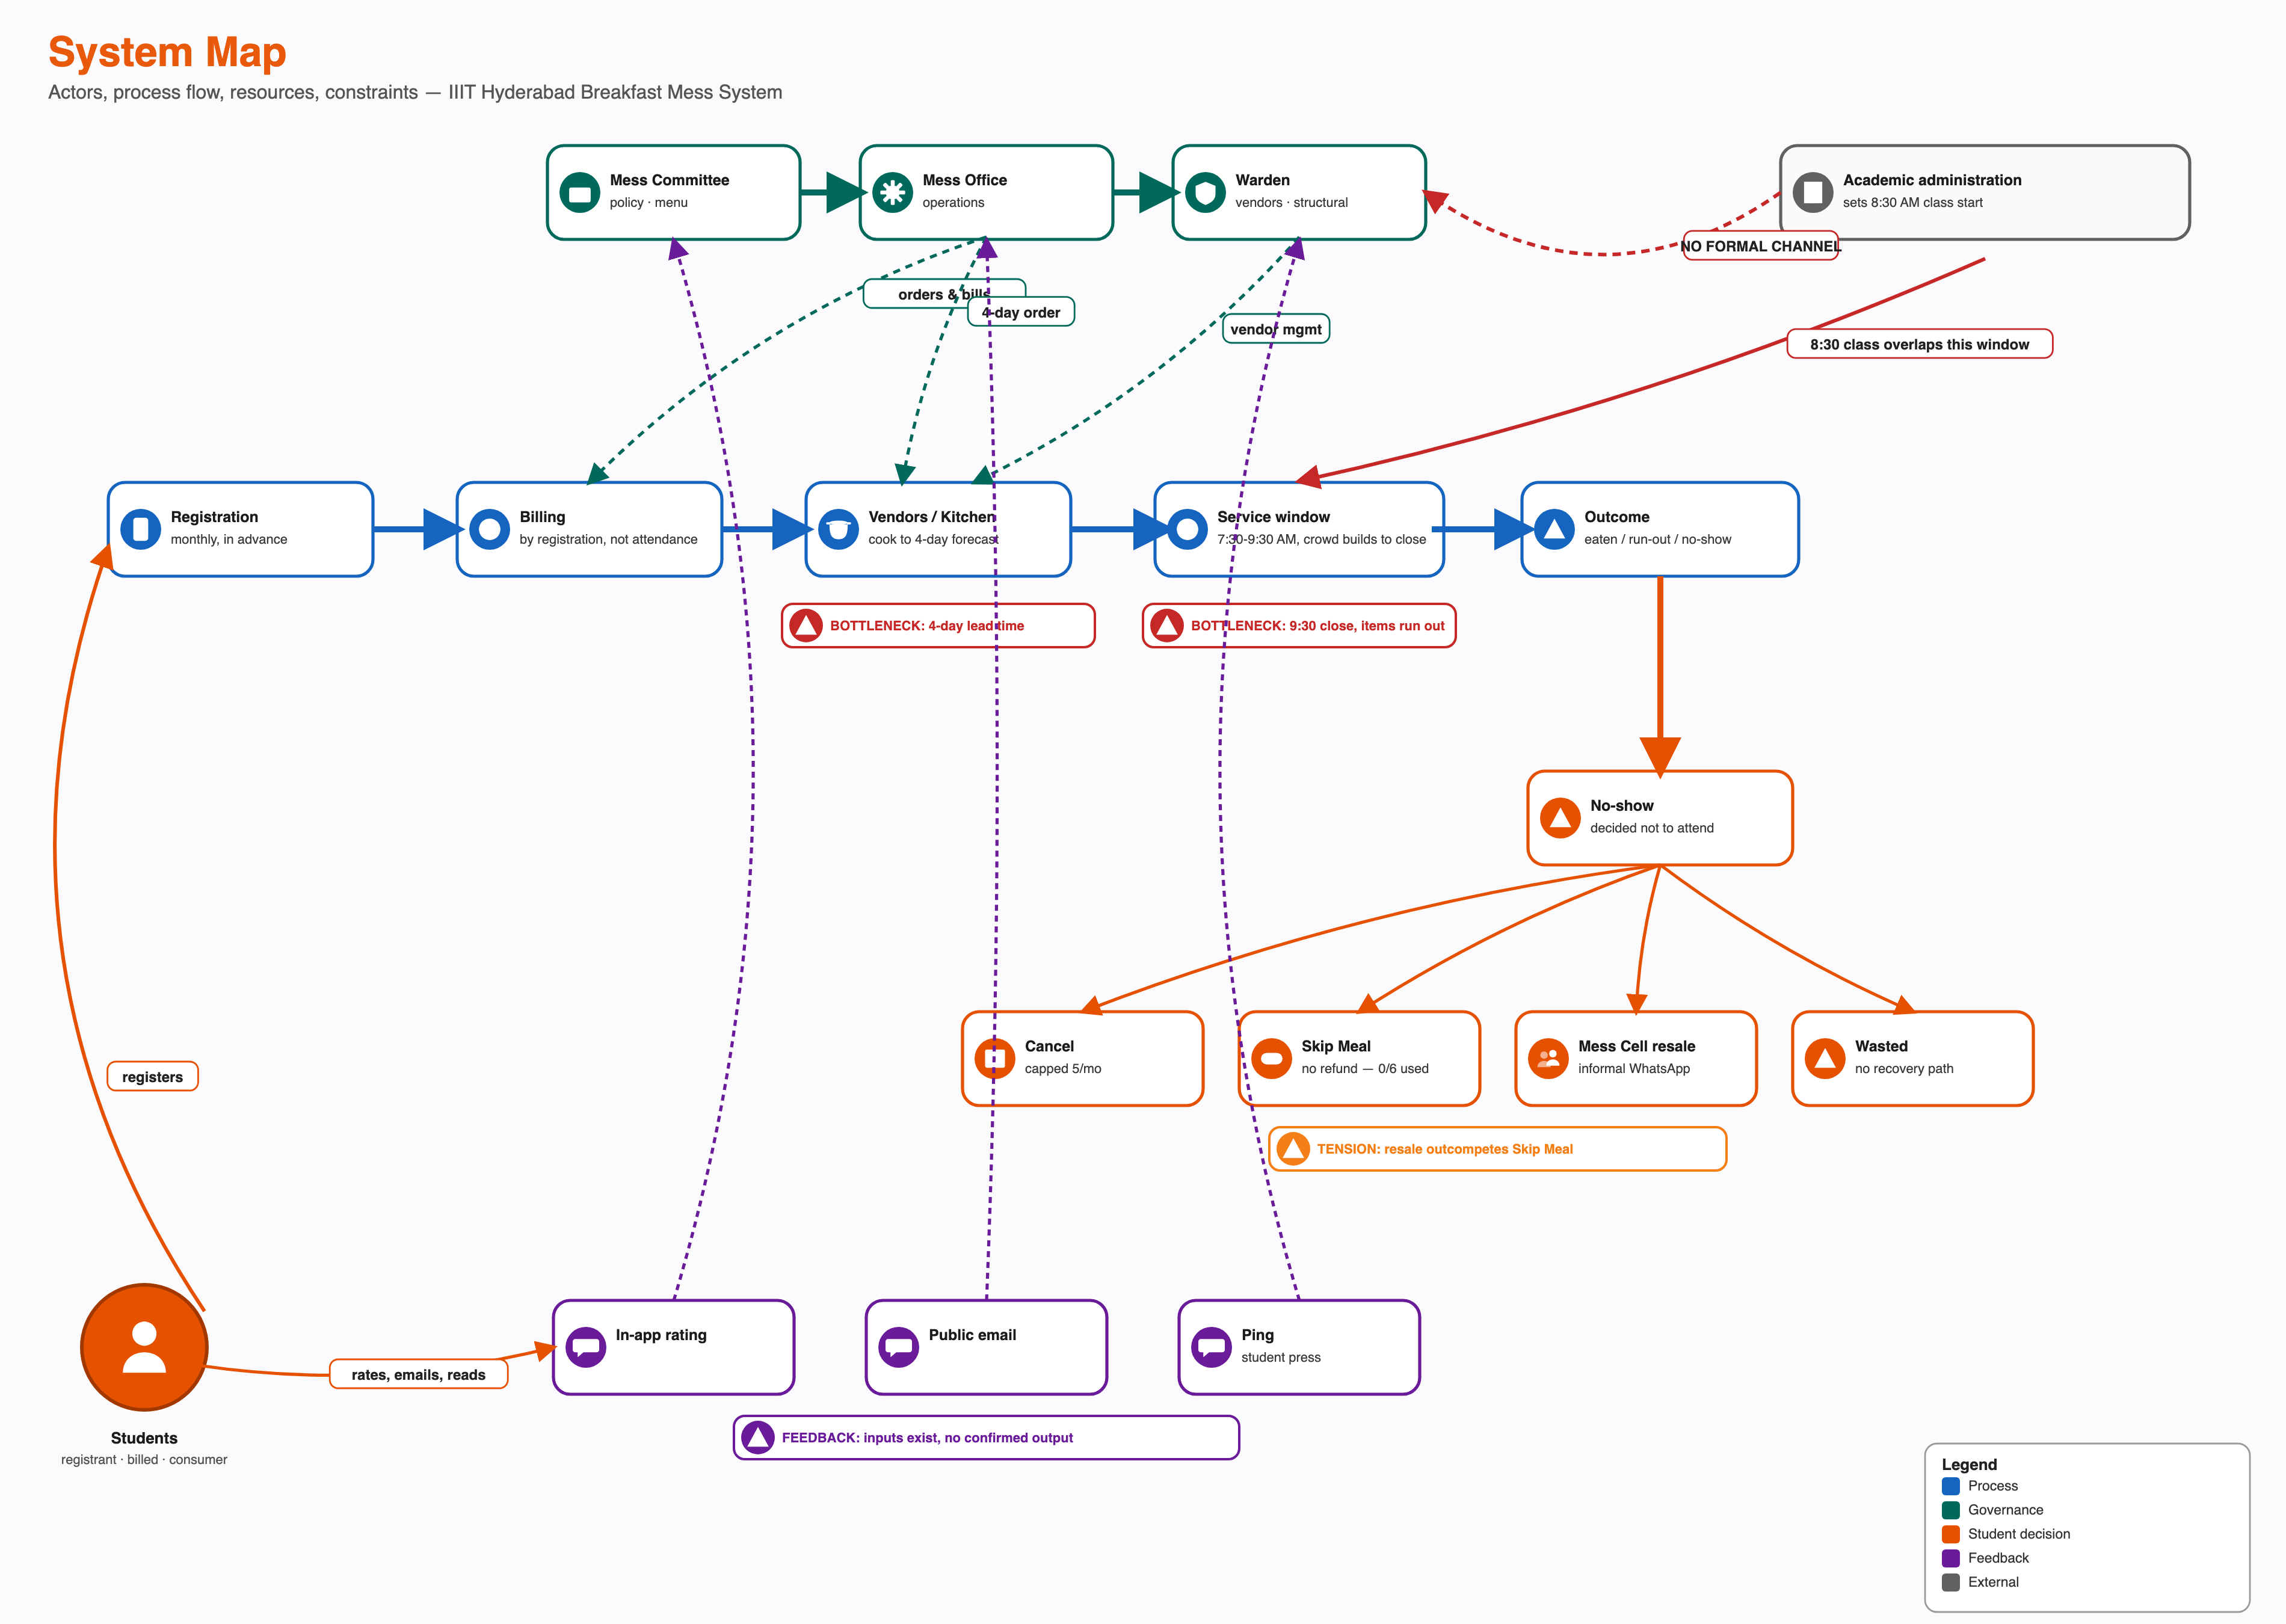
\includegraphics[width=\textwidth]{diagram1-system-map.png}
\caption{System Map, actors, process flow, resources and constraints, with bottlenecks,
tensions and feedback channels marked.}
\end{figure}

\begin{figure}[h]
\centering
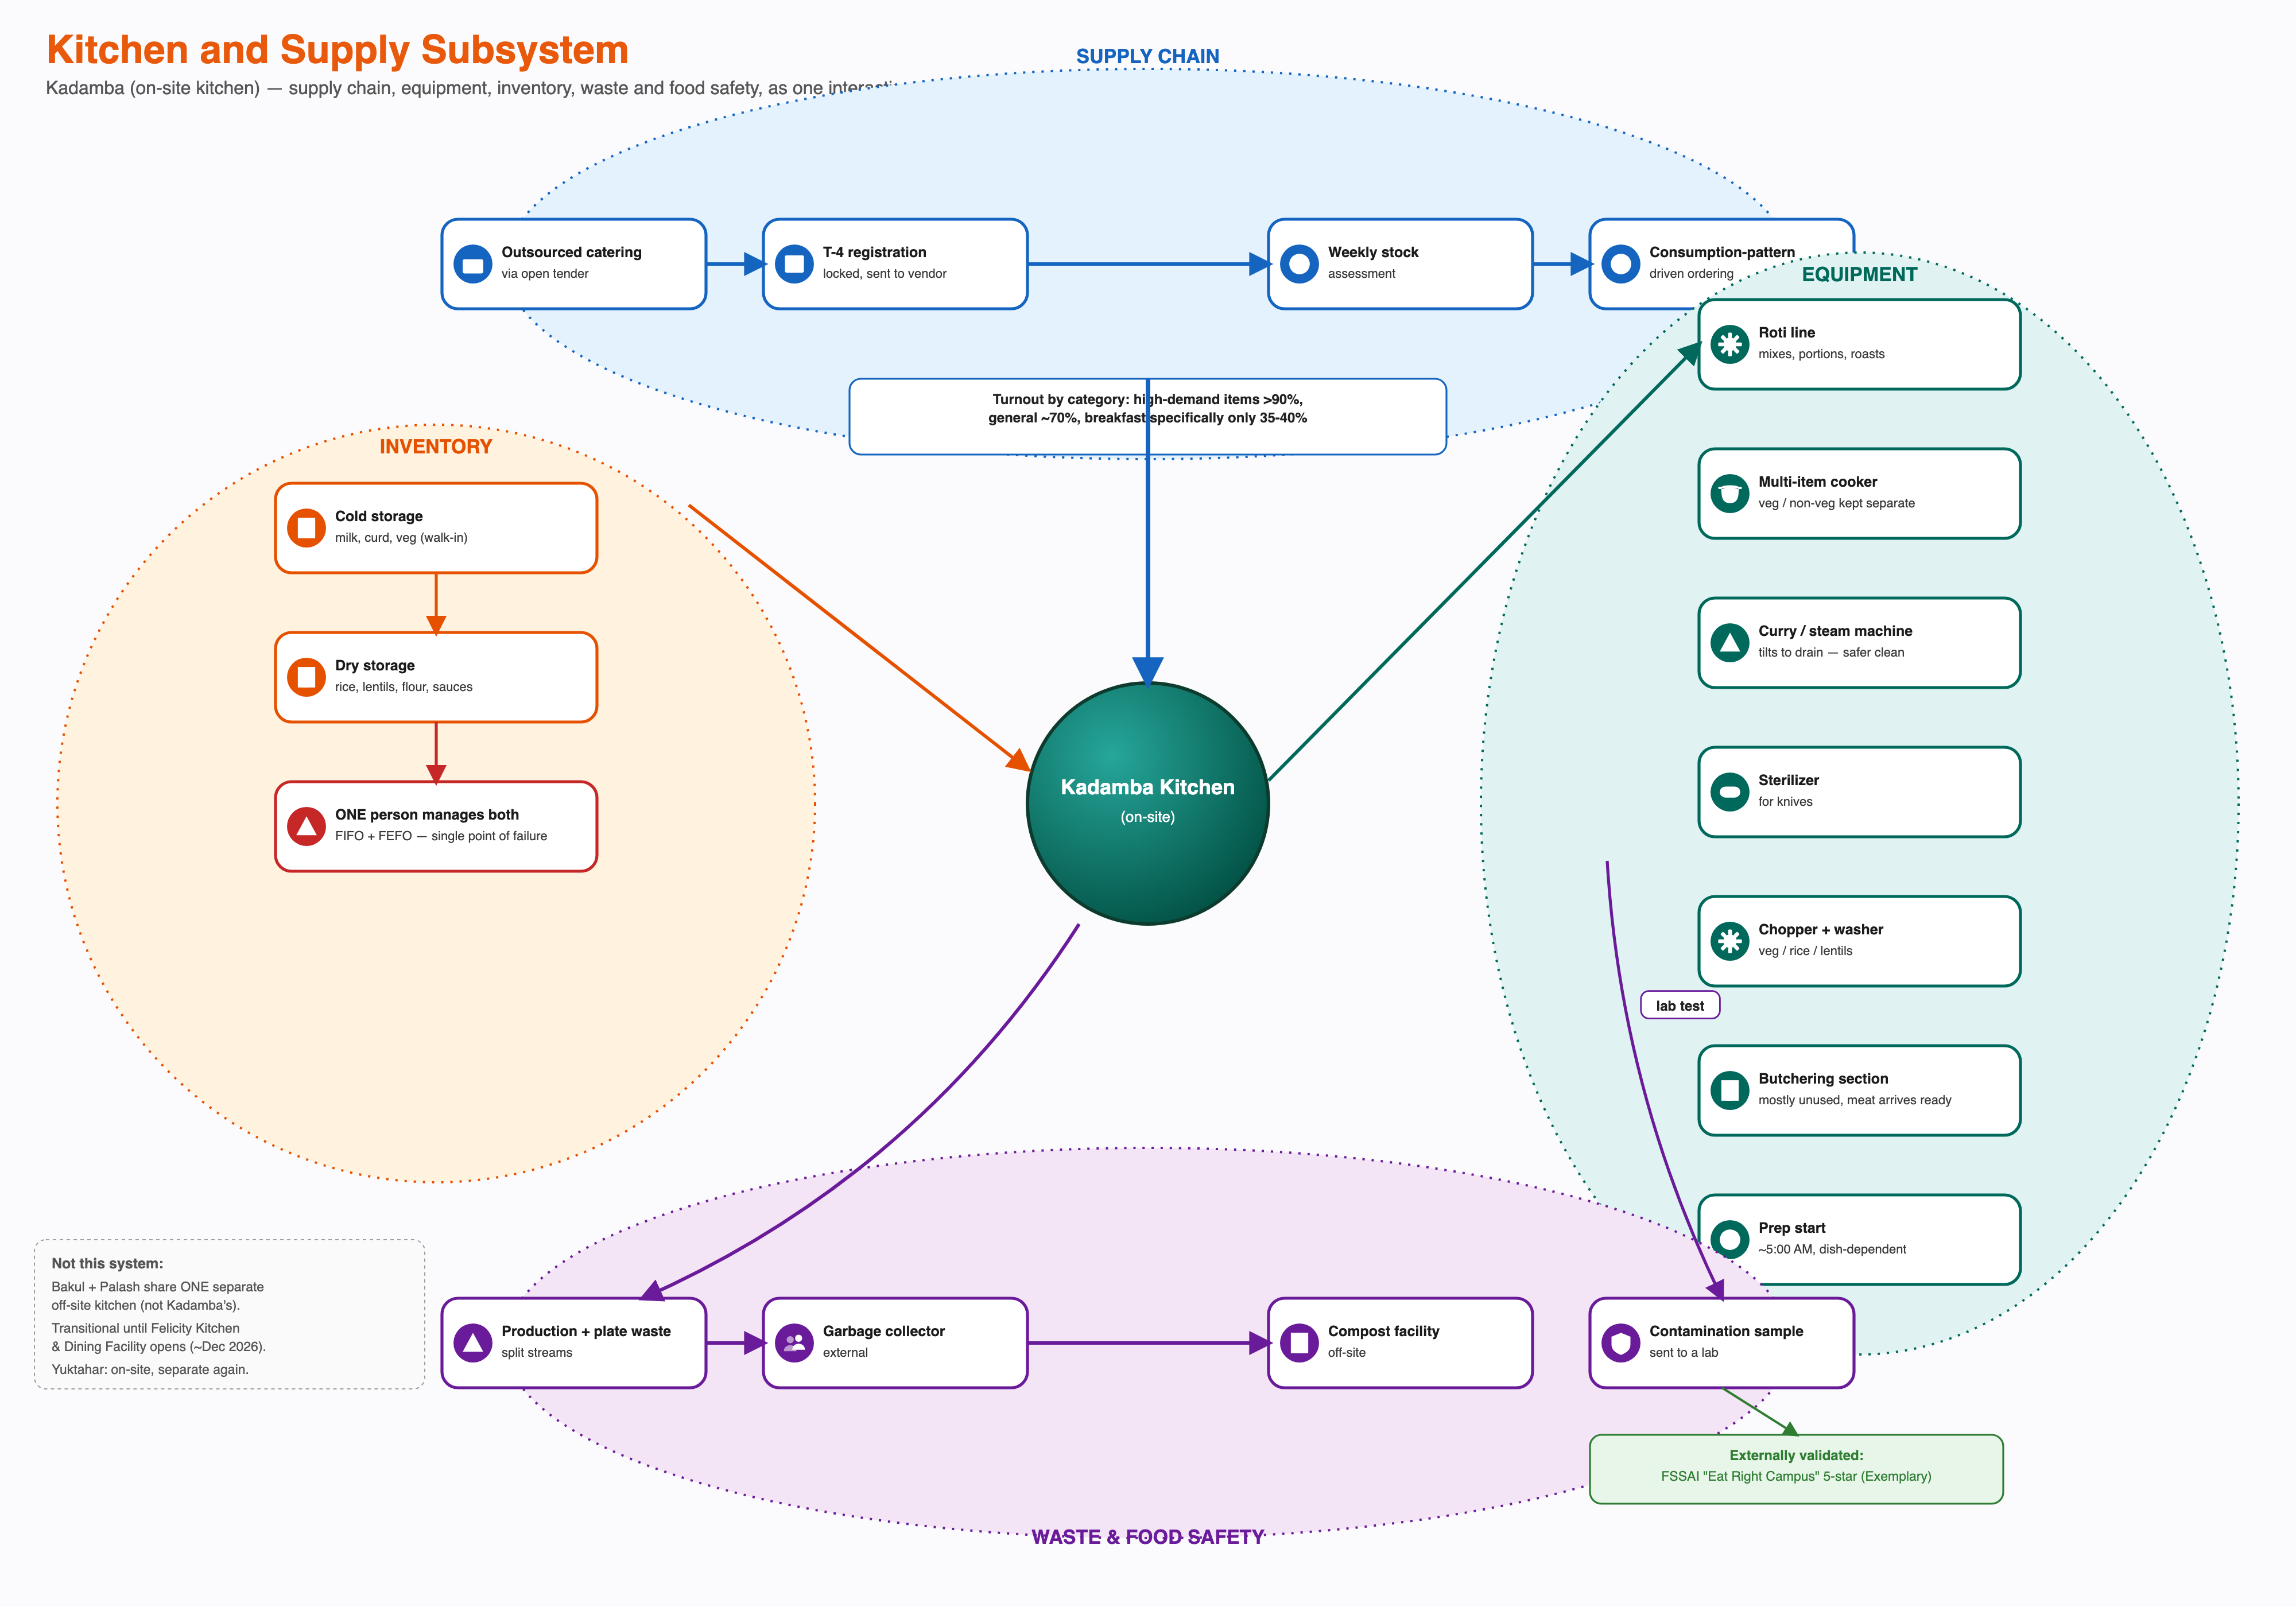
\includegraphics[width=0.92\textwidth]{diagram13-kitchen-supply-subsystem.png}
\caption{Kitchen and supply subsystem behind the vendor/kitchen node.}
\end{figure}

\subsubsection*{Three kitchens, not one}

Kadamba runs automated preparation and portions into containers out of sight. Yuktahar cooks
manually and live, and runs separate Jain and pure vegetarian lines no other hall offers. Palash
cooks nothing on site; it and Bakul are served by one outside vendor. These are three structurally
different systems, so a finding about turnout, waste or quality at one should not be assumed to
transfer to the others.

\subsubsection*{Formal and informal structure}

Low-intensity feedback goes directly to the CFS Head; high-intensity feedback escalates through the
CDS Student Council to the CDS Committee. That pathway has produced a real result: a standing
complaint about a single semester-long menu escalated and returned as a menu rotating every two
weeks, the clearest working feedback loop in this project.

Outside the formal structure sit Mess Cell, Ping (the student publication, covering mess issues
with no confirmed authority to act), and at least one unofficial registration-management tool.
Academic administration has no formal or informal relationship to any part of mess governance,
a confirmed absence, not a research gap.

\begin{figure}[h]
\centering
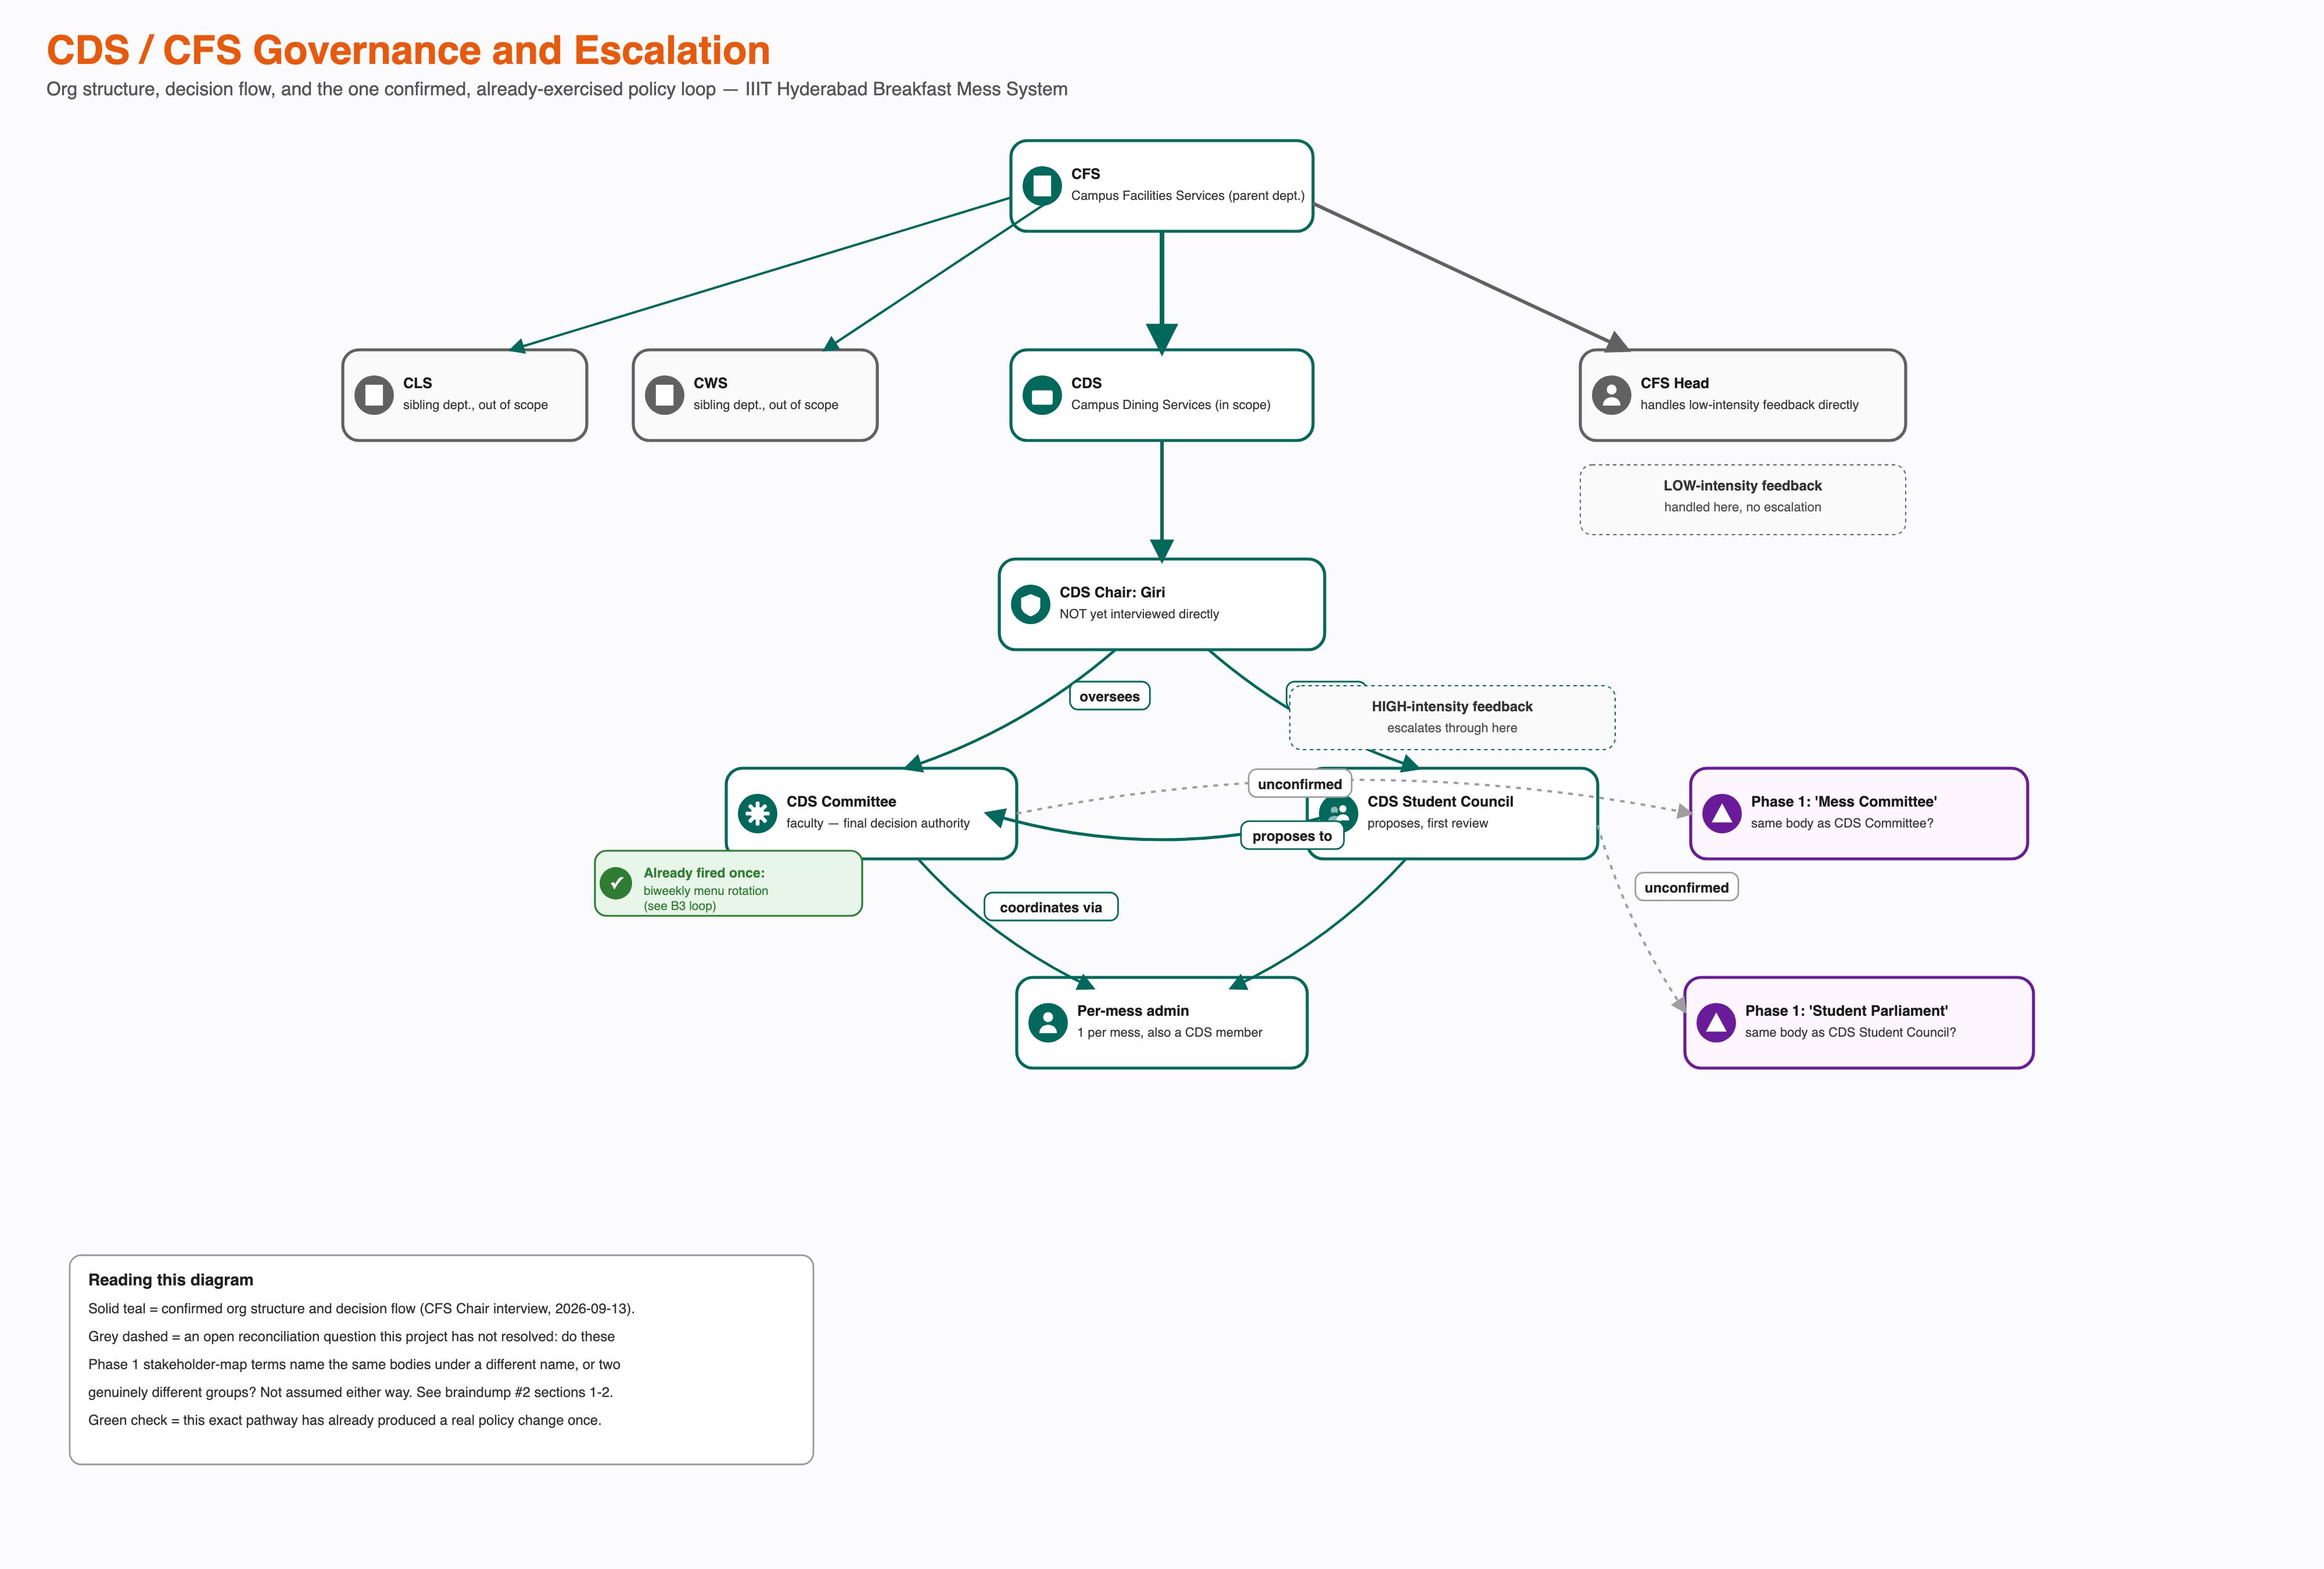
\includegraphics[width=0.85\textwidth]{diagram12-governance-escalation.png}
\caption{CDS and CFS governance and escalation pathway.}
\end{figure}

\subsubsection*{Conflicts, dependencies and bottlenecks}

Students depend on the vendor for food; the vendor depends on no individual student. The vendor
depends on CDS for a four-day forecast. CDS depends on students registering accurately, but nothing
in billing requires that accuracy, the one relationship where the party with less to lose
controls an input the other cannot replace. Kadamba's entire inventory depends on one person with
no named backup.

Four bottlenecks are confirmed: the four-day ordering lock, which no same-day signal can reach; the
9:30 close against a crowd cresting just before it; the absence of any channel between Academic
administration and mess governance; and waste never being measured by volume, so it cannot function
as a signal for anything.

\subsection{Deliverable 2: Causal Loop / Feedback Analysis}
\deliv{2}{Causal Loop / Feedback Analysis, reinforcing and balancing loops tested for closure}

Ten candidate feedback mechanisms were tested. A mechanism counts as a loop only if its last step
causally returns to affect its first. Five close; five are real mechanisms that stop partway and are
named as such rather than presented as loops.

\begin{figure}[h]
\centering
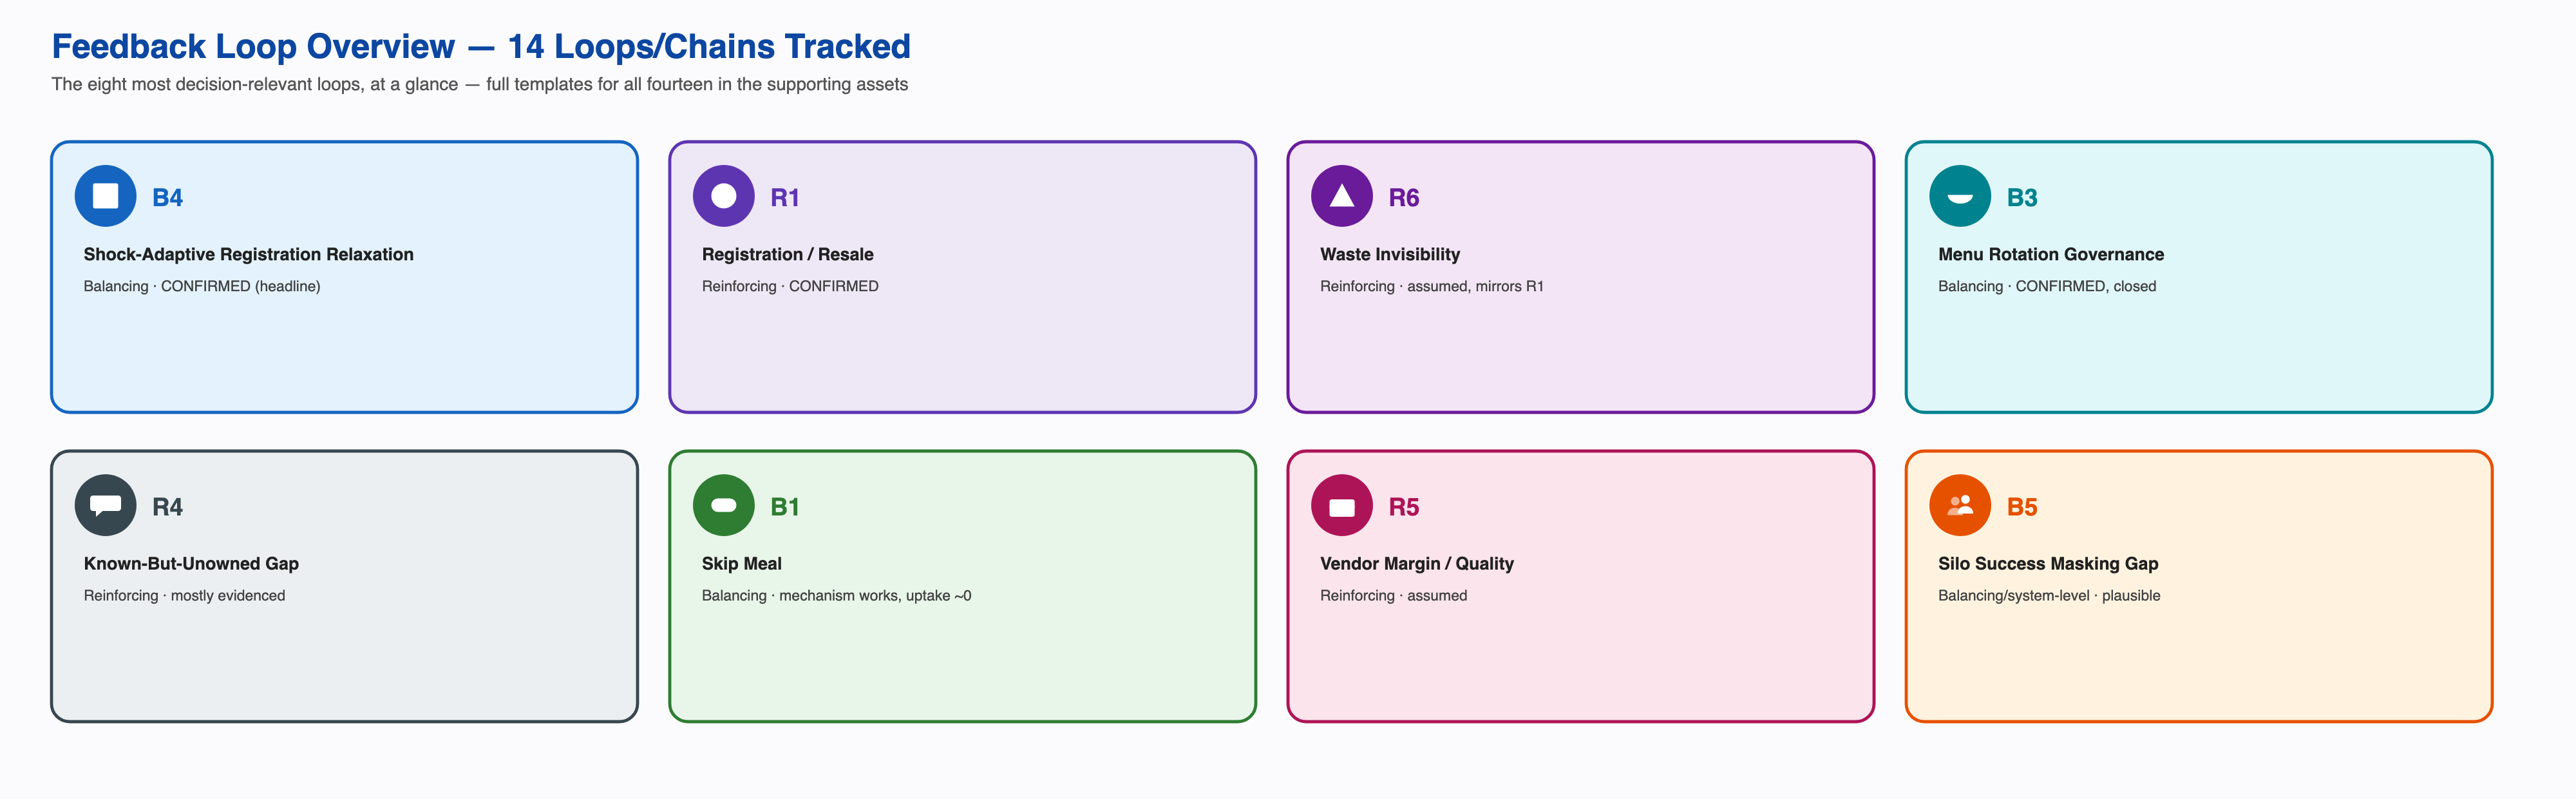
\includegraphics[width=0.95\textwidth]{diagram17-loop-overview-dashboard.png}
\caption{Overview of all tested feedback mechanisms and their closure status.}
\end{figure}

\subsubsection*{Loops that close}

\textbf{Registration and resale (reinforcing).} Loose registration feeds the Mess Cell resale
market; resale removes the financial sting of an unused registration; that softer cost plausibly
makes loose registration feel safe again. Most links are confirmed by direct quotes; the final link
is a reasonable but unconfirmed assumption.

\begin{figure}[h]
\centering
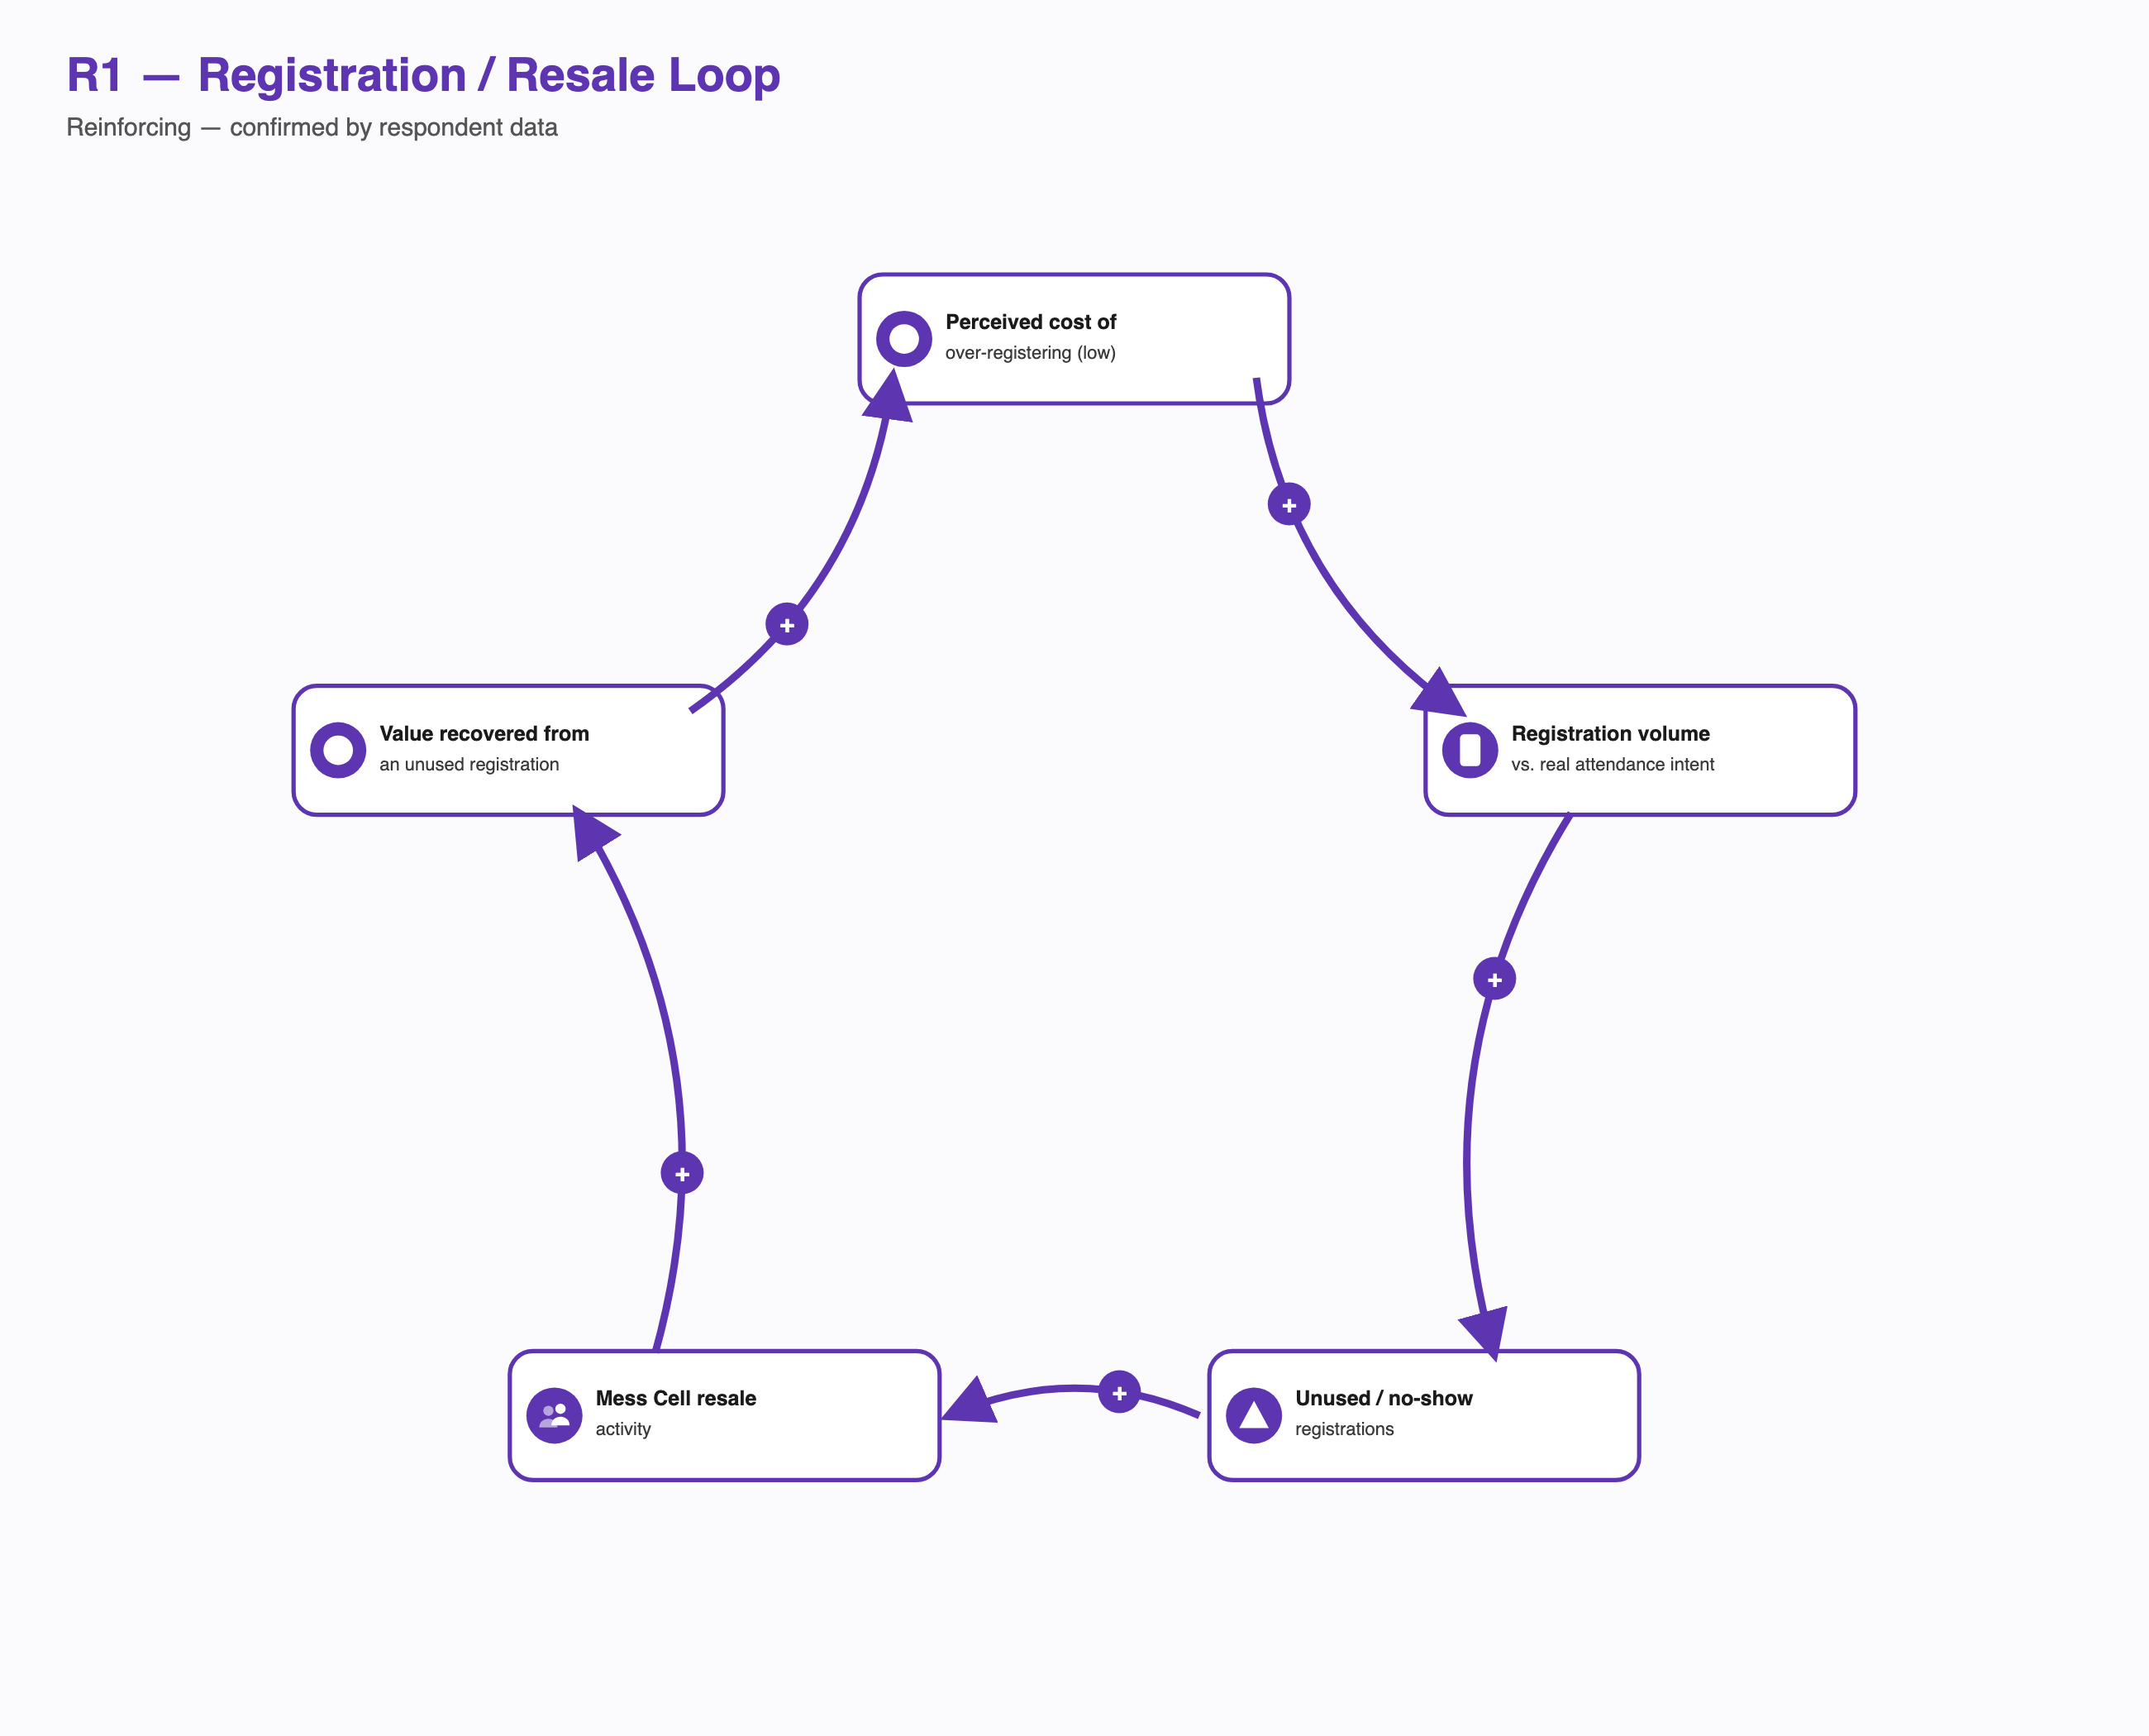
\includegraphics[width=0.72\textwidth]{diagram4-cld-r1-resale.png}
\caption{Registration and resale loop.}
\end{figure}

\textbf{Menu rotation governance (balancing).} Menu fatigue drove feedback, feedback escalated
through the Student Council, the Committee approved a rotation, and variety reduced fatigue. Every
step confirmed directly by the CFS Chair, the cleanest closed loop in the system.

\begin{figure}[h]
\centering
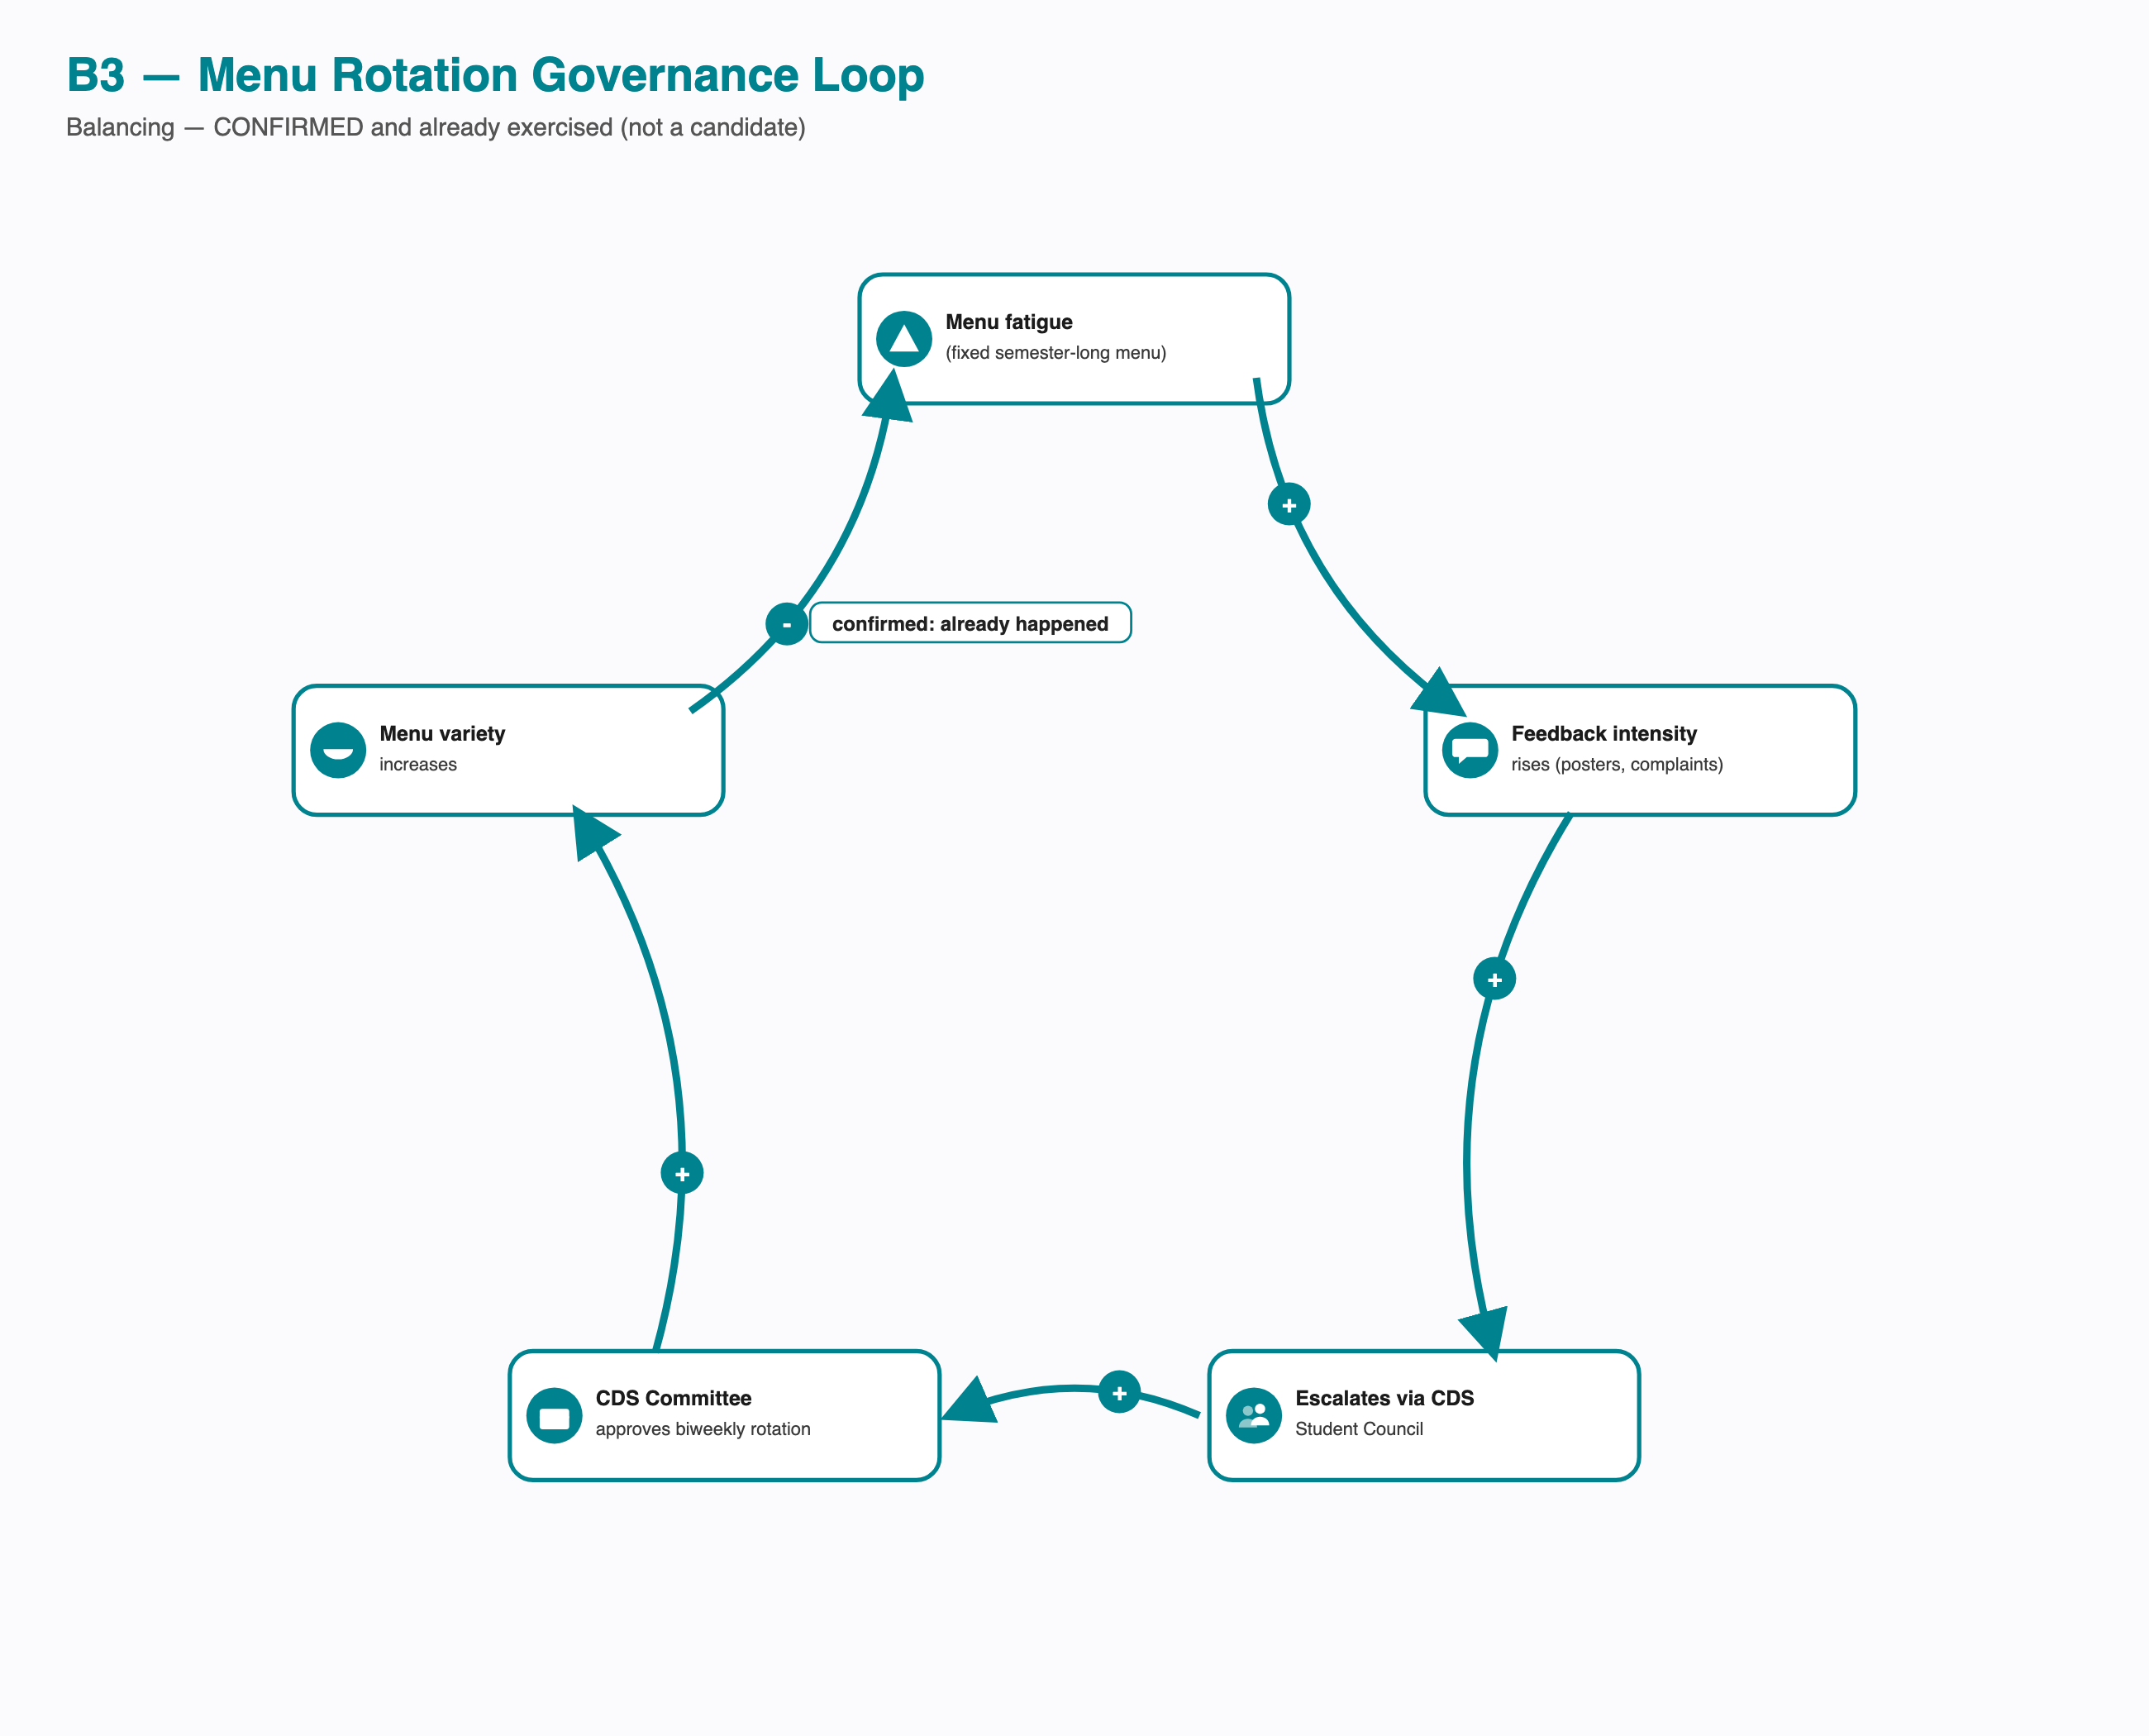
\includegraphics[width=0.72\textwidth]{diagram10-cld-b3-menu-rotation.png}
\caption{Menu rotation governance loop.}
\end{figure}

\textbf{Shock-adaptive registration relaxation (balancing).} Uncertainty rises, registration
compulsion relaxes, billing follows real attendance, the vendor absorbs more uncertainty, and
confidence in keeping the relaxed model drops, so it reverts. Trigger and mechanism confirmed;
whether it closes as a genuine loop or is an on/off switch tied to the calendar remains open.

\begin{figure}[h]
\centering
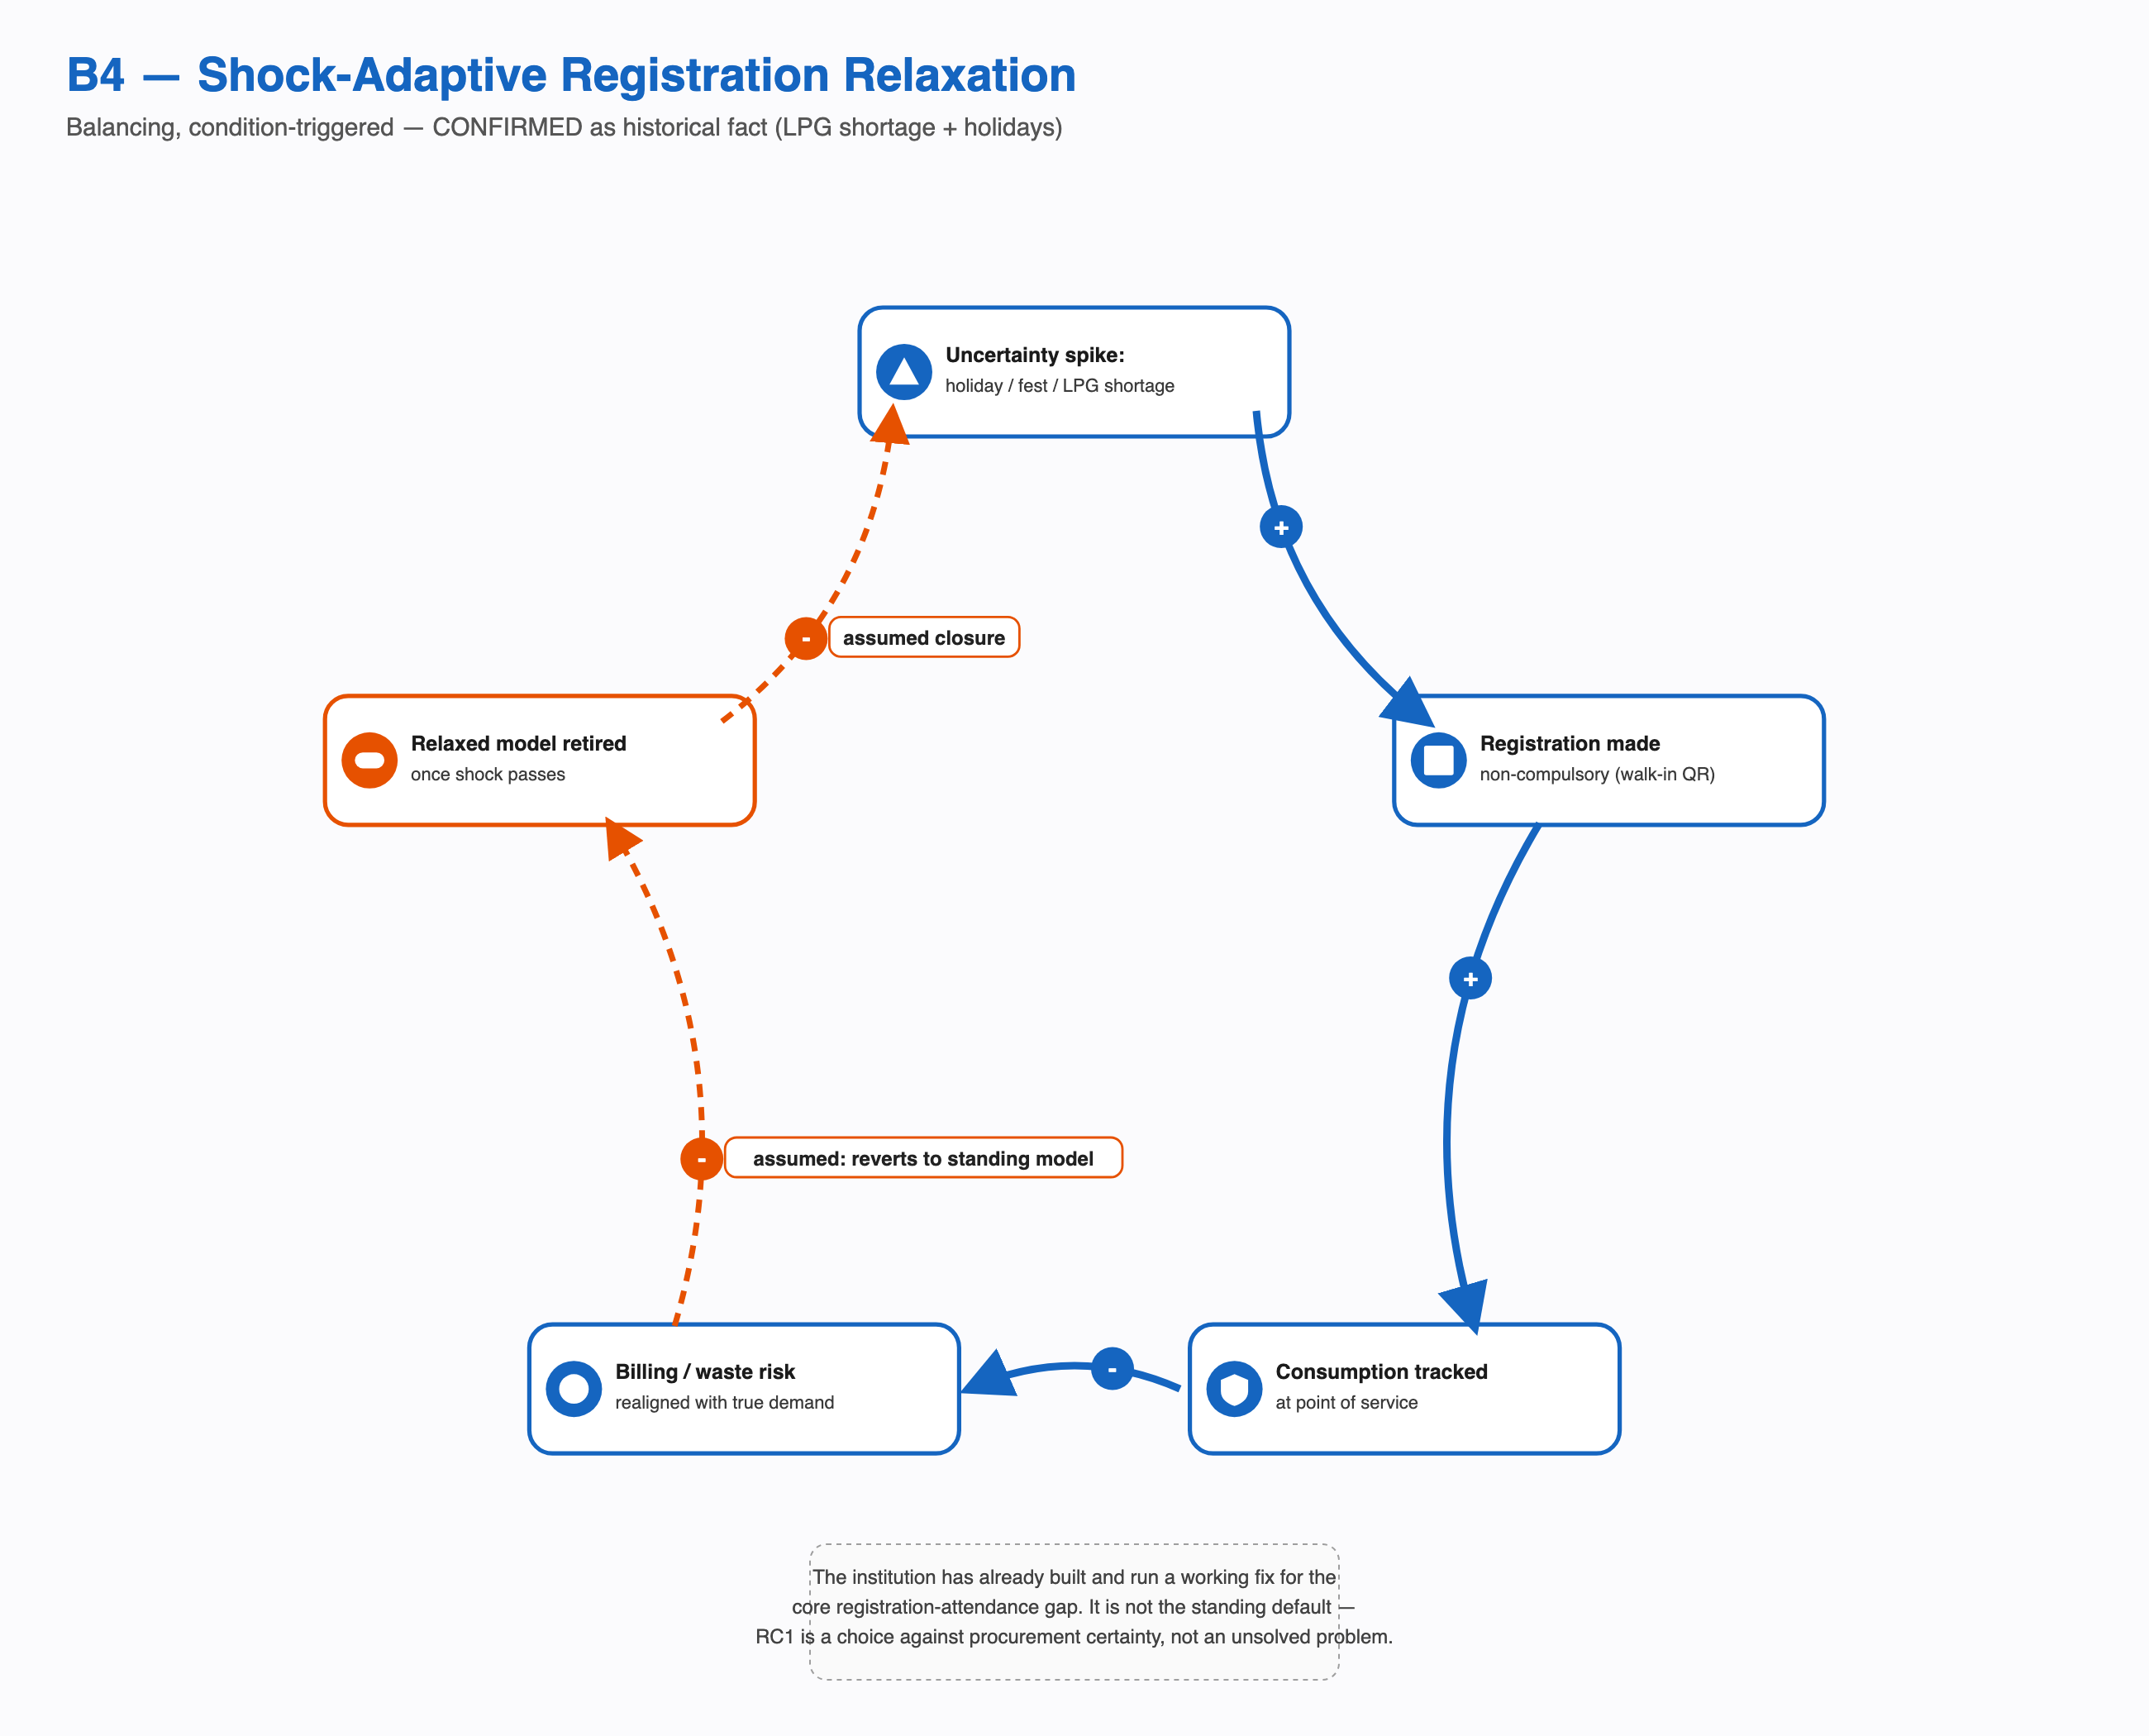
\includegraphics[width=0.72\textwidth]{diagram14-cld-b4-shock-adaptive.png}
\caption{Shock-adaptive registration relaxation loop.}
\end{figure}

\textbf{Kadamba scarcity concentration (reinforcing).} Popularity drives defensive month-long
registration, which keeps Kadamba scarce. The middle link is confirmed by direct quote; the closing
link is weak, since the only available description of a crowded Kadamba is negative.

\textbf{Waste invisibility (reinforcing).} Waste is composted competently enough that it never
becomes visible pressure to fix anything upstream. Composting is confirmed; that composting
specifically suppresses the pressure is assumed.

\subsubsection*{Mechanisms that do not close}

\begin{longtable}{L{0.34\textwidth}L{0.60\textwidth}}
\toprule
\textbf{Mechanism} & \textbf{Why it is not a loop} \\
\midrule
\endhead
Skip Meal & Reaches the kitchen and adjusts same-week cooking, but nothing returns to change whether
a student uses it. A working one-way mechanism with near-zero uptake. \\
Menu transparency and selective skipping & A self-identified second-order risk of the rotation fix,
with no evidence of anything looping back. \\
Attendance pressuring vendor quality & The link that would close it is confirmed missing: vendor
payment tracks registration, not attendance. \\
Capacity redistribution to Bakul/Palash & The opposite occurs, scarcity concentrates demand on
Kadamba rather than dispersing it. \\
Known-but-unowned gap worsening over time & Nothing shows it worsening cycle over cycle. A stable
stuck state, not a spiral. \\
\bottomrule
\end{longtable}

\begin{figure}[h]
\centering
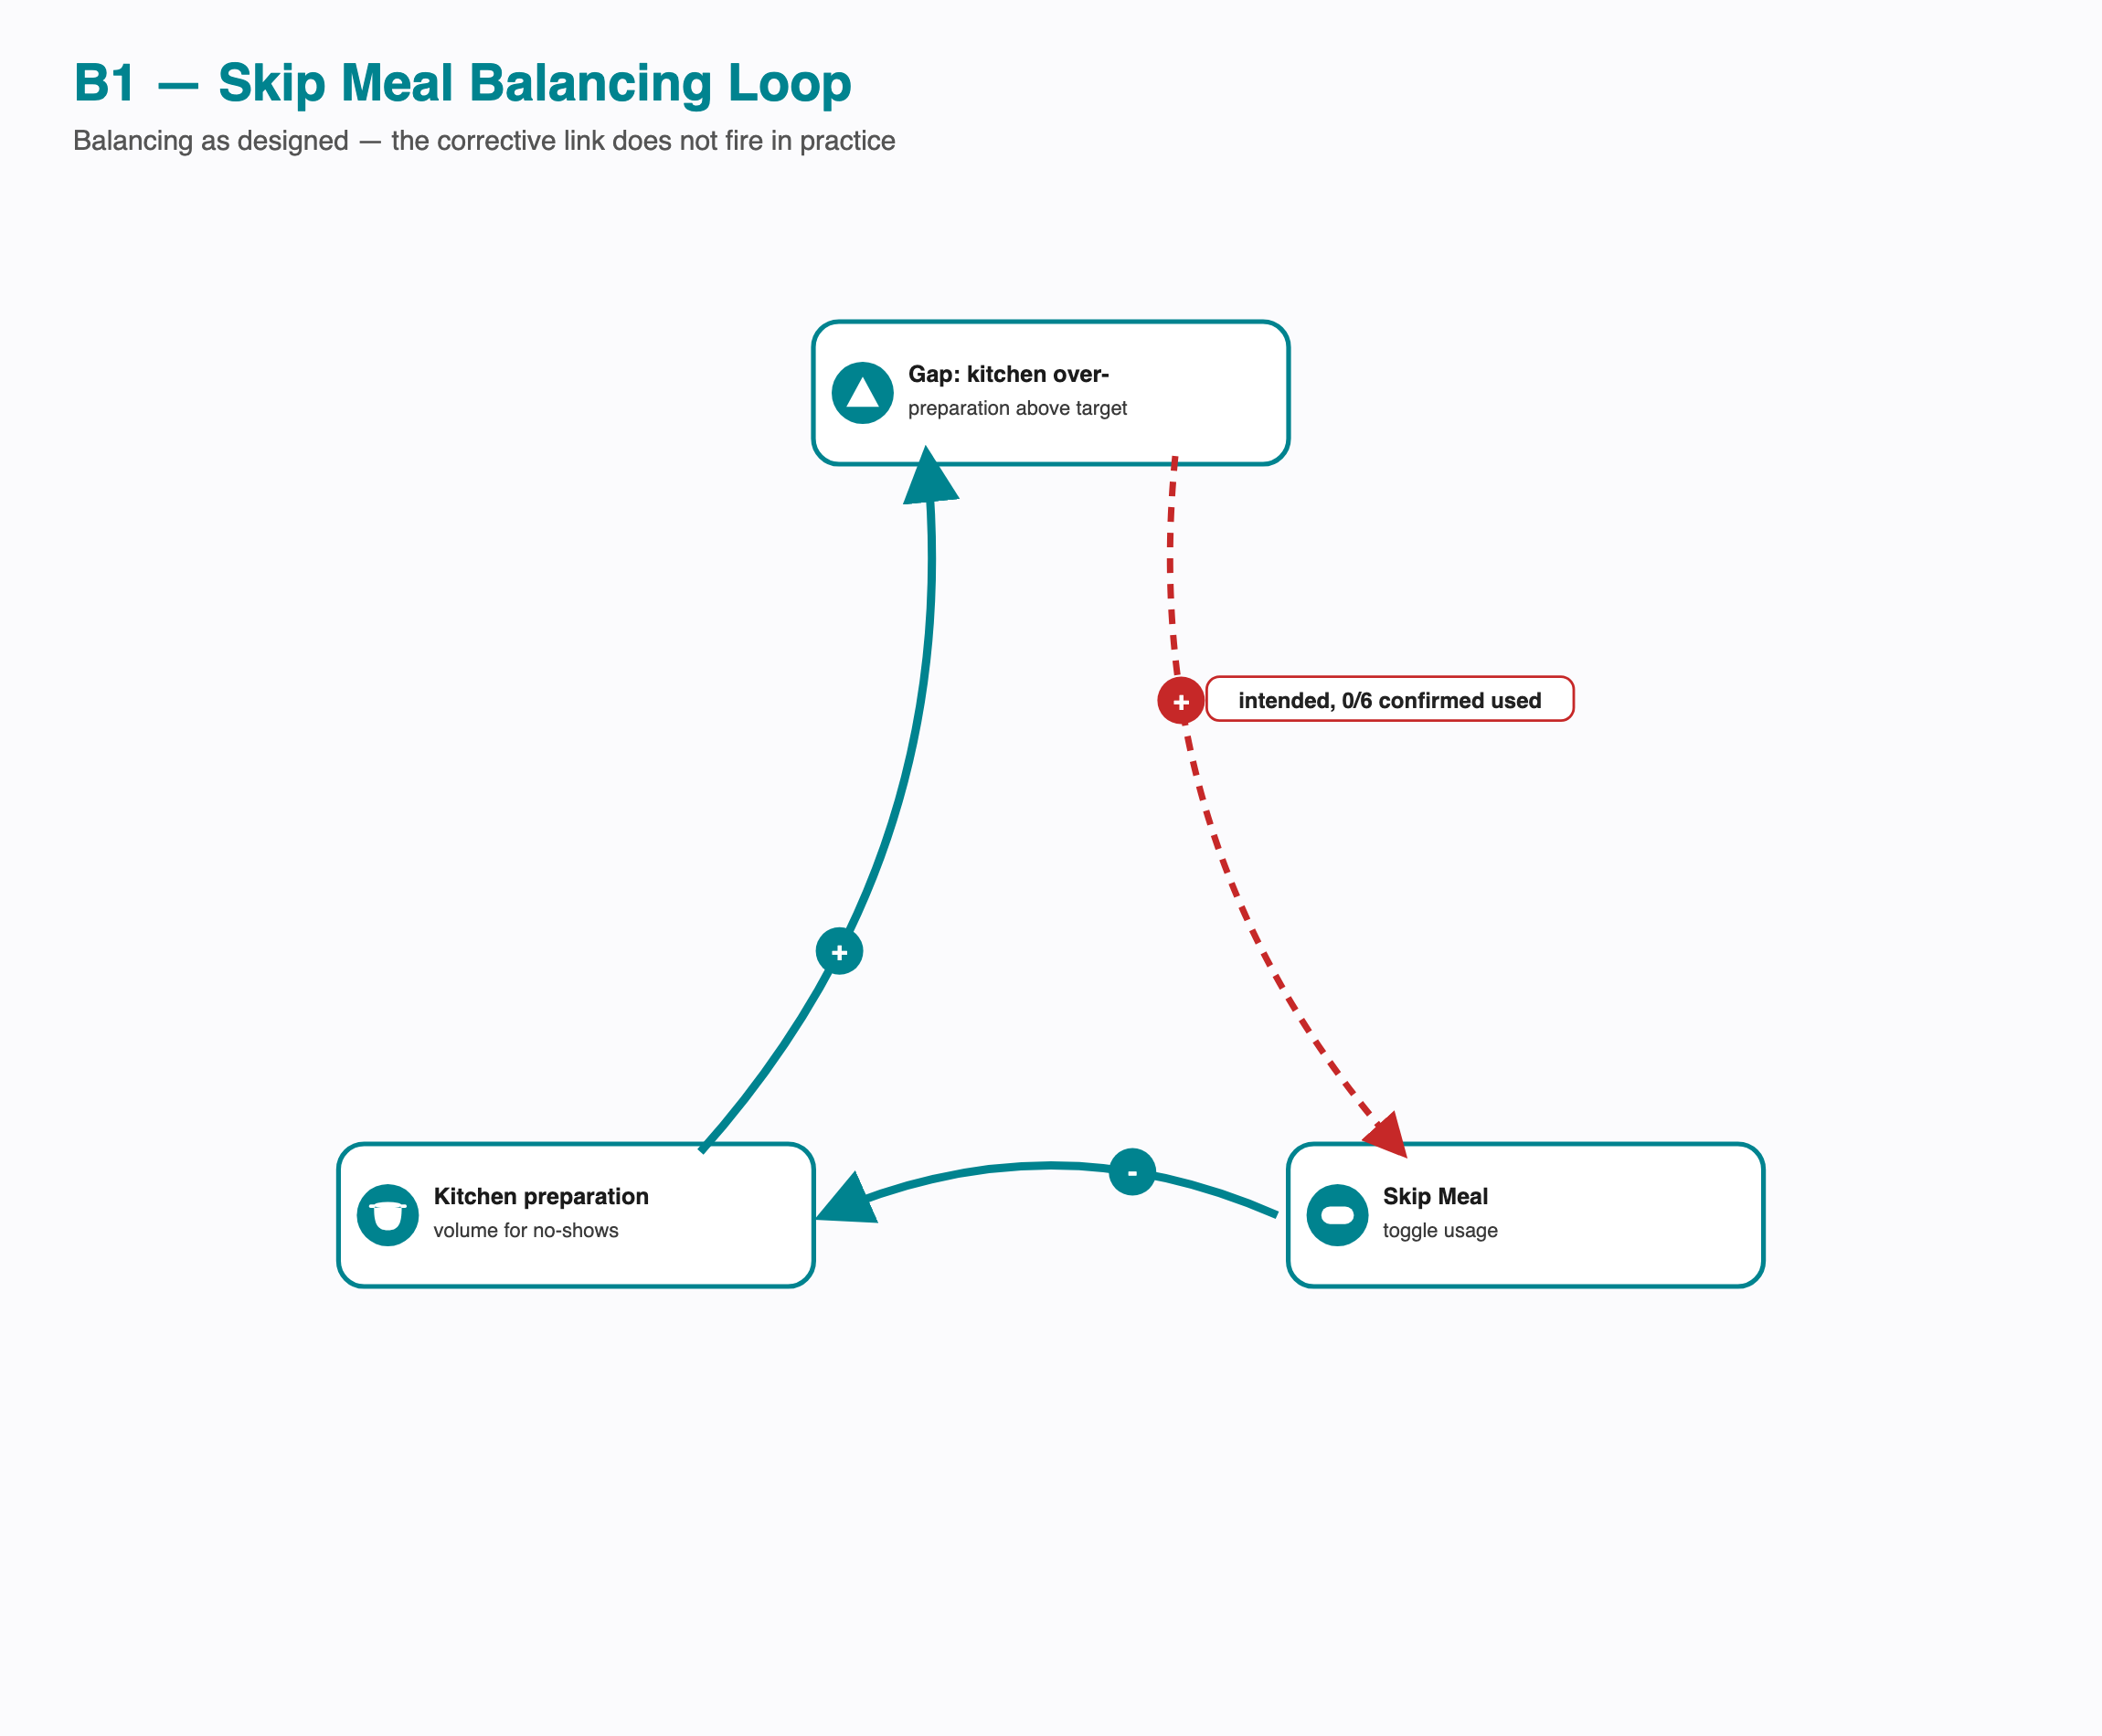
\includegraphics[width=0.72\textwidth]{diagram5-cld-b1-skipmeal.png}
\caption{Skip Meal, a functioning one-way mechanism rather than a closed loop.}
\end{figure}

\newpage
%============================================================
\section{Activity 7: Identify Systemic Patterns and Root Causes}

\textbf{Purpose:} move from symptoms to the underlying structures and mechanisms producing the
problem.

\deliv{3}{Systemic Problem Analysis: patterns, structures, feedback loops and root causes}

\subsection{The Iceberg Model, six chains}

Six areas were traced from event to belief. An event is one thing that happened; a pattern is what
keeps happening; a structure is the rule producing the pattern; a mental model is the belief holding
the structure up.

\begin{figure}[h]
\centering
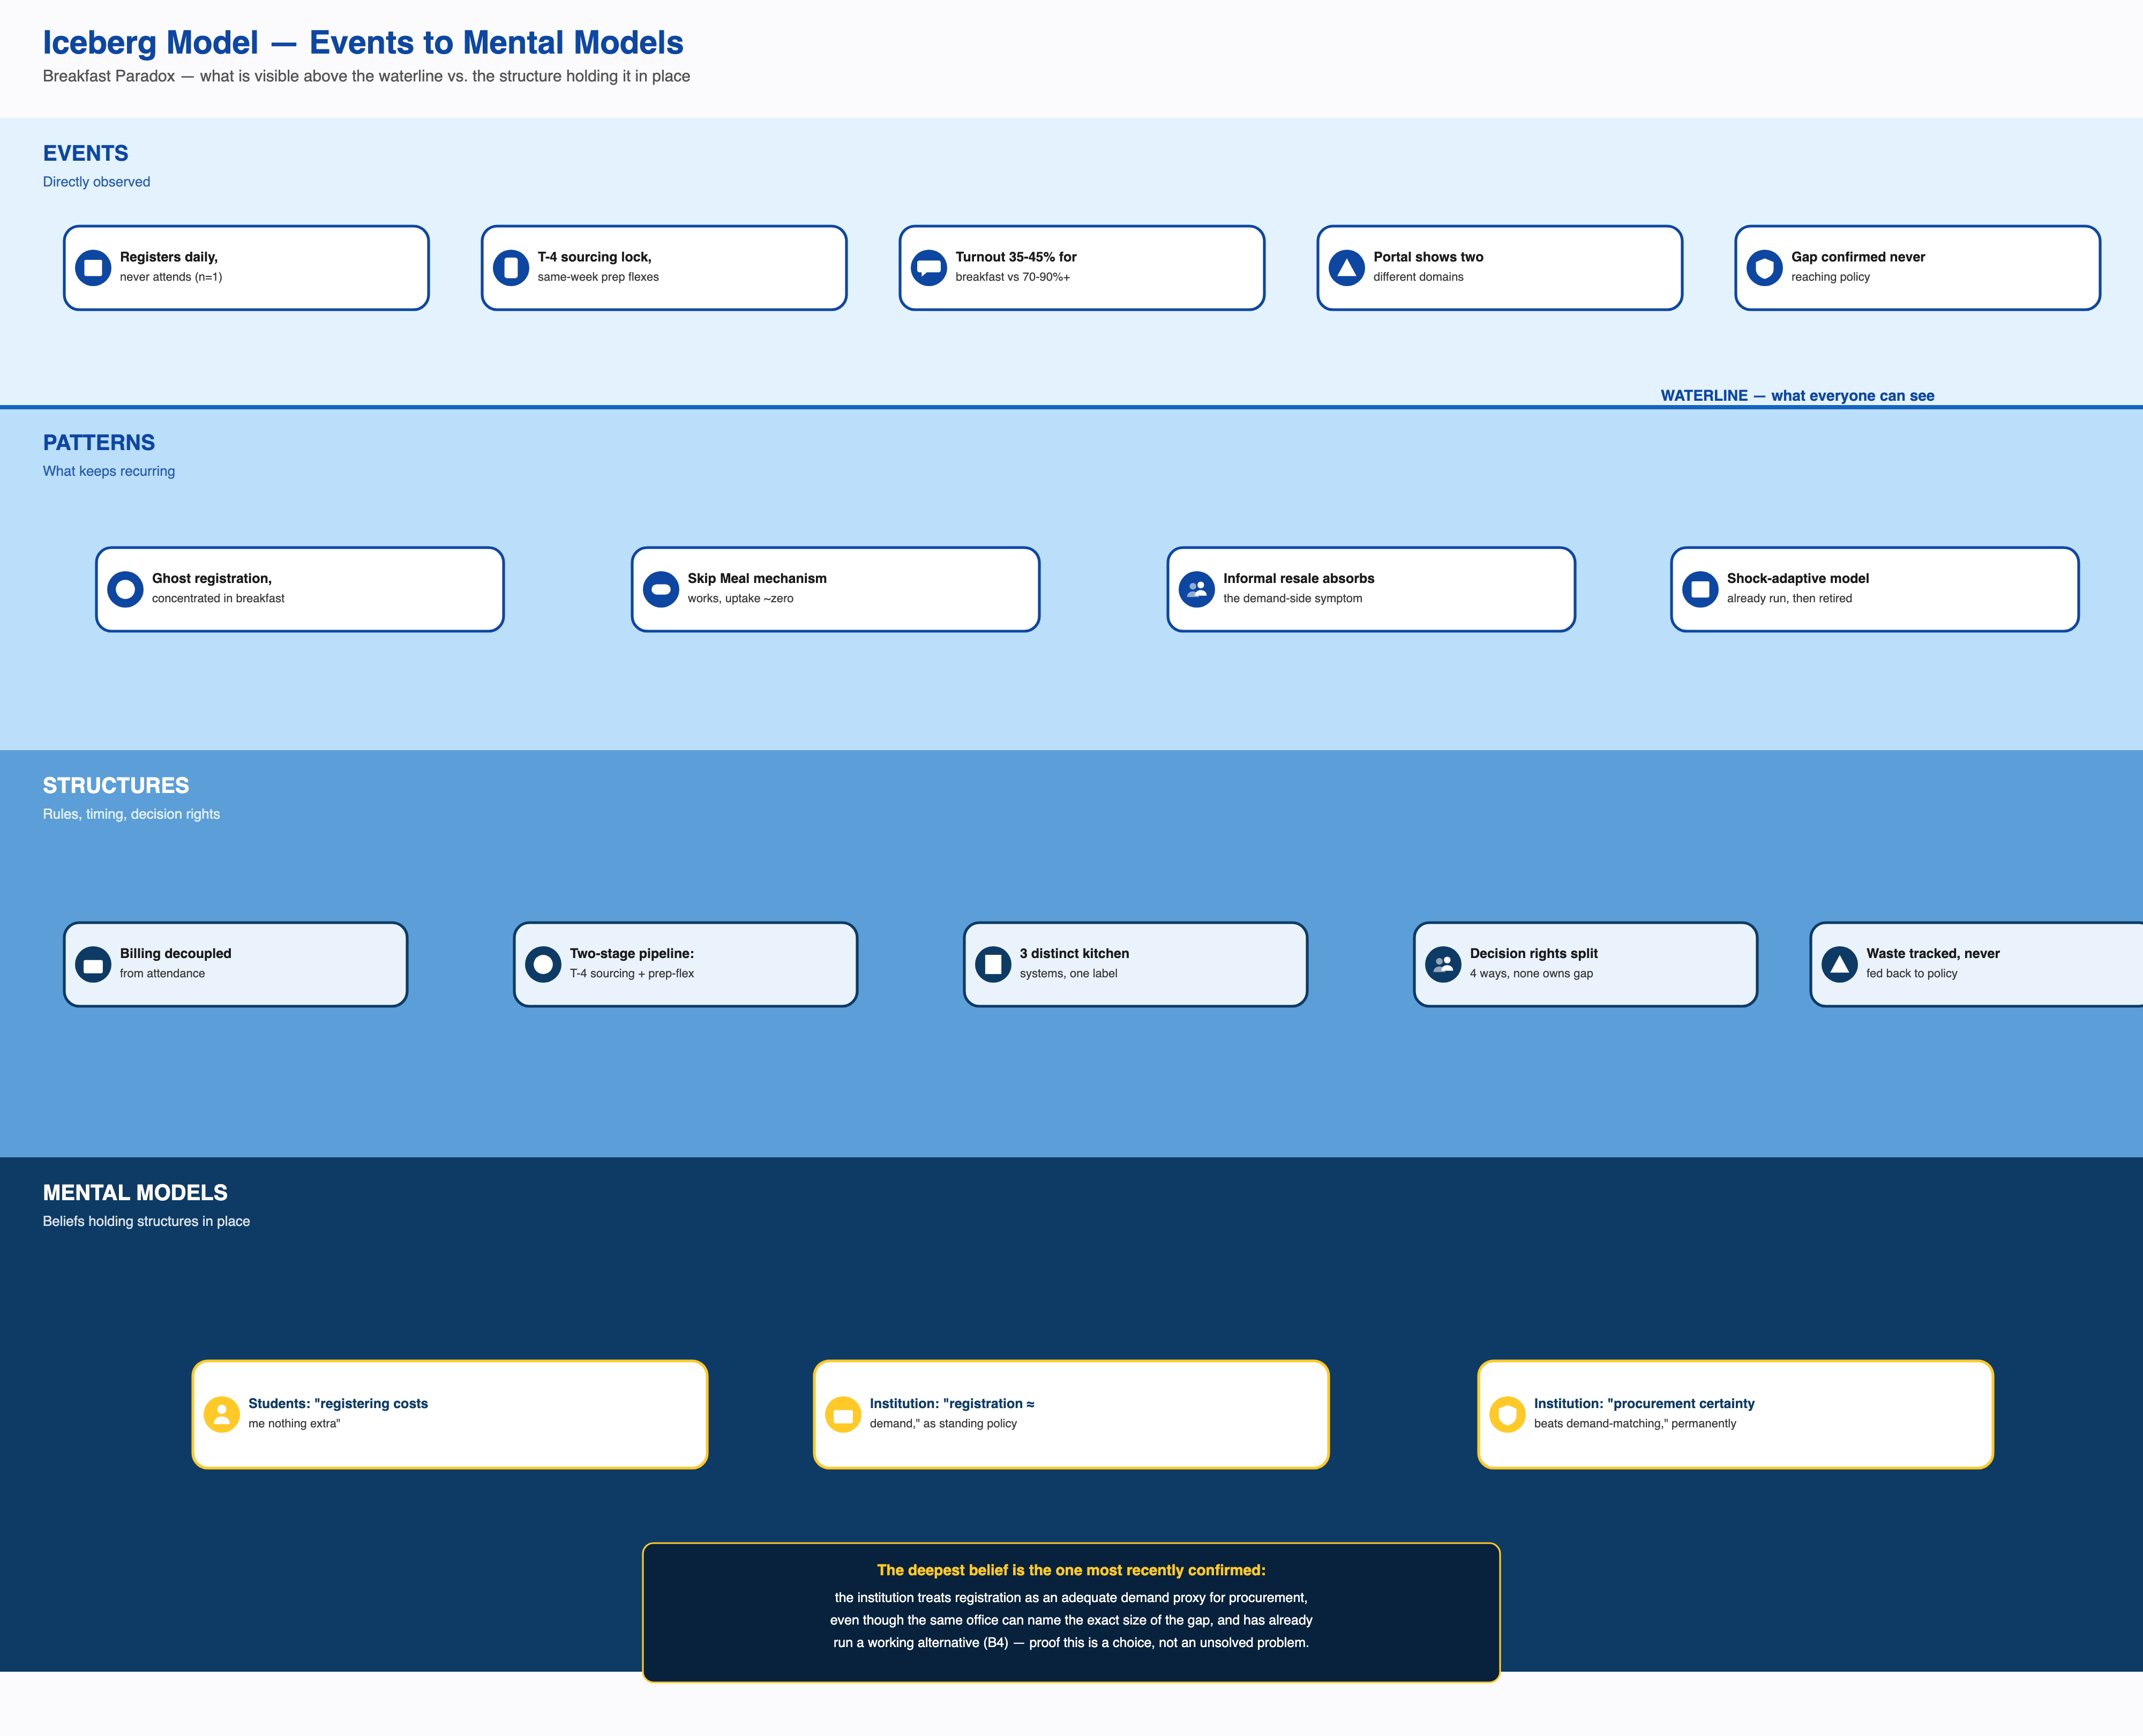
\includegraphics[width=0.9\textwidth]{diagram15-iceberg-model.png}
\caption{Iceberg Model across the six traced chains.}
\end{figure}

\begin{longtable}{L{0.20\textwidth}L{0.36\textwidth}L{0.38\textwidth}}
\toprule
\textbf{Chain} & \textbf{Key structure} & \textbf{Key mental model} \\
\midrule
\endhead
1. Register and don't show up & Billing tracks registration, not attendance; Skip Meal returns
nothing; walk-in priced 70--90\% higher & Registration count is an adequate demand proxy; a
registration already made costs nothing to leave unused \\[4pt]
2. Food runs out before close & One average consumption figure applied across all items; four-day
order lock; one person managing inventory & Procurement certainty matters more than matching food
to real demand \\[4pt]
3. Complaints ignored until forced & No confirmed committee sign-off required for operational
change; four separate decision owners & Operational decisions are the office's alone to make;
reducing its own workload justifies a rule change \\[4pt]
4. A working fix, switched off & The vendor's four-day lock requires a knowable headcount; nothing
exists to evaluate whether a temporary fix should become standing & Attendance-based billing is
acceptable only as an emergency measure \\[4pt]
5. Menu rotation and its shadow & A real escalation path with authority at the end of it; menu now
posted two weeks ahead & Menu variety is worth a policy change; more transparency is automatically
good (now being revised) \\[4pt]
6. Some of this isn't a problem & Breakfast is a low-companionship meal; only one hall offers
separate Jain and pure vegetarian lines & Sleep outweighs a booked breakfast; the system assumes
everyone should default into breakfast \\
\bottomrule
\end{longtable}

\subsection{Structural root causes}

Three causes recur across the chains, tested against four criteria each: is it structural, does it
explain multiple independent patterns, would the pattern collapse without it, and is it evidenced.

\textbf{RC1, Billing is decoupled from attendance.} The financial obligation is created at
registration, not consumption. This explains the incentive to over-register, Skip Meal's non-use,
why a cancellation cap is needed, why Mess Cell exists, and why a vendor might quietly prefer the
current model. Unusually, its counterfactual has actually been run: when billing tracked attendance
during the shortage and holidays, the gap closed. Confirmed.

\textbf{RC2, Decision rights are fragmented.} Menu, kitchen execution, academic scheduling and
billing policy sit with four separate owners, none holding both the knowledge and the authority.
This is why the CFS Chair can state the gap's exact size and it has still never reached a
registration or billing policy discussion, and why a proven fix has never been evaluated for
standing adoption. Confirmed.

\textbf{RC3, Attention triggers on complaint intensity, not data severity.} Escalation routes
high-intensity feedback to the Committee and low-intensity feedback to the CFS Head. Both respond
to how loudly a problem is felt, neither to how much it costs. Menu fatigue, sharp, daily,
individually felt, travelled the full pathway and produced a policy change. The registration
gap, quiet, monthly, diffuse, and already quantified, never has. Mechanism confirmed; the
causal generalisation is a candidate.

A fourth, lower-confidence factor: the vendor is paid the same whether or not students attend, so
it has little independent reason to push for change. Assumed, pending contract terms.

\begin{figure}[h]
\centering
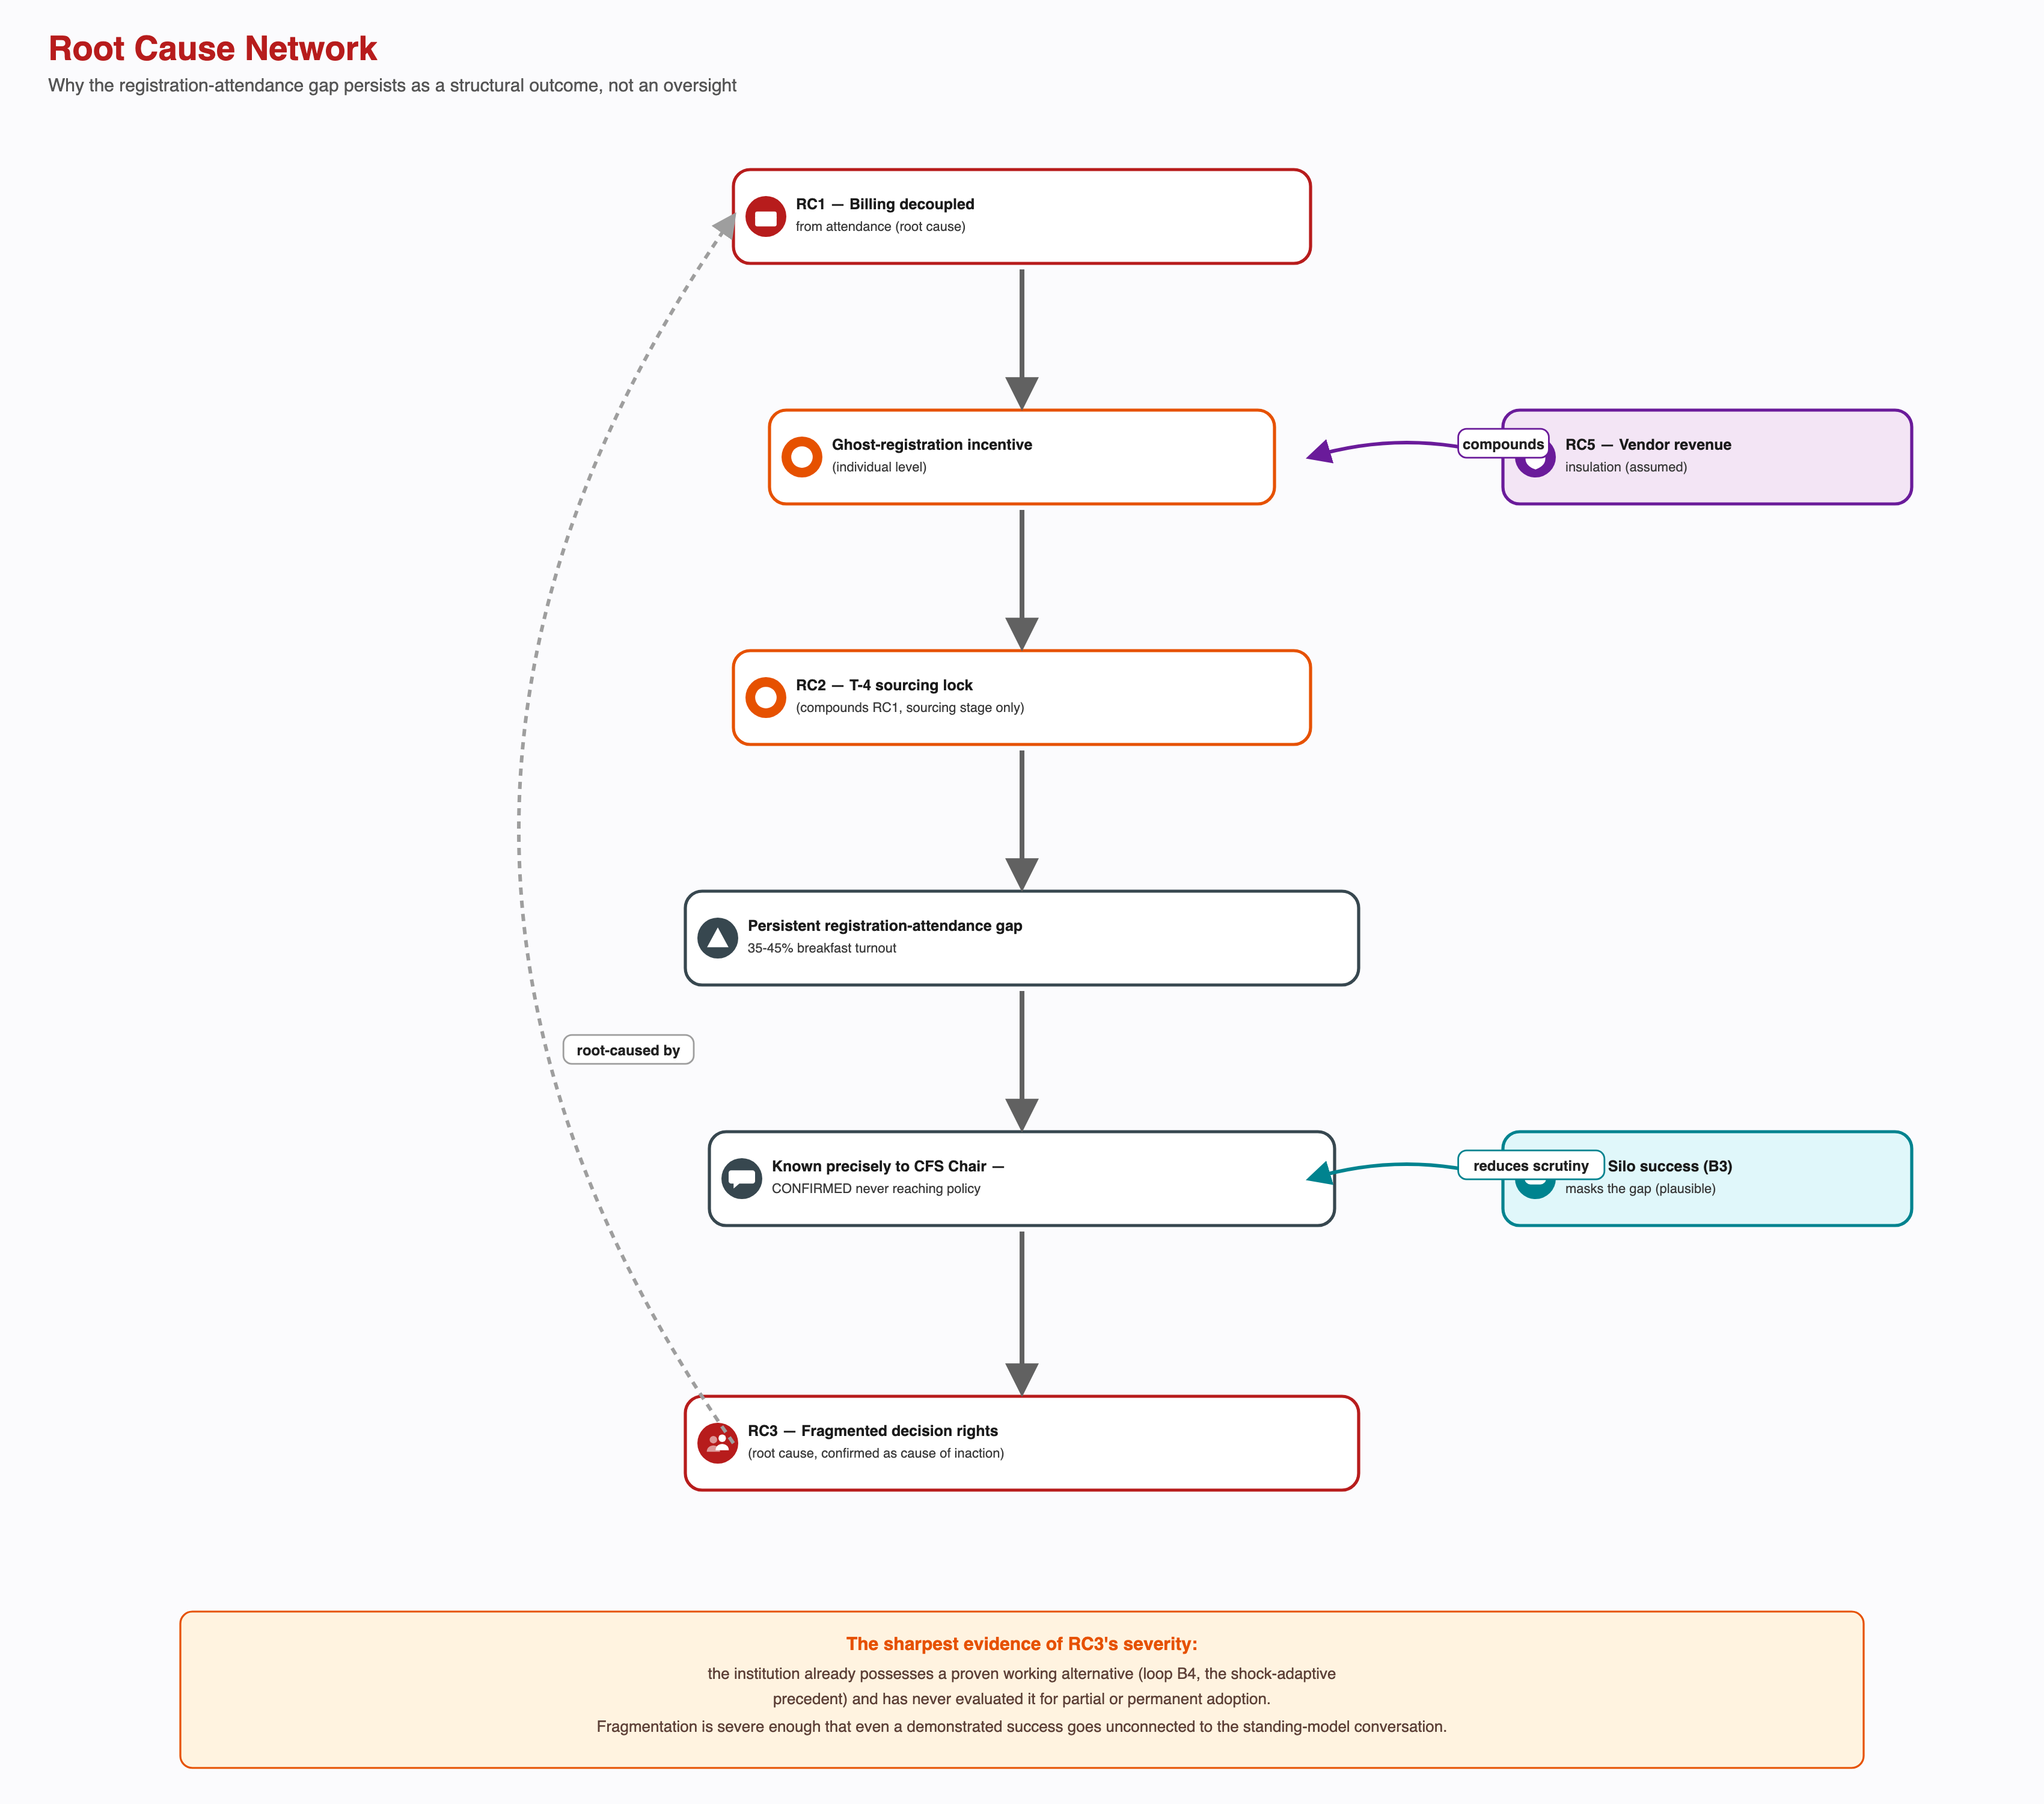
\includegraphics[width=0.92\textwidth]{diagram16-root-cause-network.png}
\caption{Root cause network, how RC1, RC2 and RC3 interact and compound.}
\end{figure}

\subsection{Unintended consequences}

\begin{longtable}{L{0.24\textwidth}L{0.28\textwidth}L{0.42\textwidth}}
\toprule
\textbf{Rule} & \textbf{Intended function} & \textbf{Unintended consequence} \\
\midrule
\endhead
Cancellation cap & Limit uncancelled no-shows & Constrains a behaviour some students don't
reliably perform anyway; tightening plausibly pushes traffic into silent no-shows \\[4pt]
Walk-in markup & Discourage same-day uncertainty & Universal monthly advance registration,
inflating counts independent of intent \\[4pt]
Skip Meal, no refund & Reduce kitchen waste & Near-zero uptake, so it may not be reducing waste in
practice at all \\[4pt]
Menu rotation & Fix menu fatigue & Created a way to plan skipping on disliked menu days \\[4pt]
Composting and food safety & Keep the mess clean and compliant & Waste never becomes a number
anyone must explain, so it cannot create upstream pressure \\[4pt]
Outsourcing the kitchen & Save cost, modernise hygiene & Vendor paid on registration regardless of
turnout, removing its reason to care about the gap \\
\bottomrule
\end{longtable}

\subsection{System archetypes}

Eleven standard archetypes were tested. Five hold: \textbf{Shifting the Burden} (resale substituting
for a billing fix; composting substituting for measuring waste), \textbf{Limits to Growth} (Kadamba's
demand hitting a capacity ceiling, answered by building Bakul rather than removing the limit),
\textbf{Success to the Successful} (Kadamba's scarcity pulling further demand toward itself),
\textbf{Rule Beating} (registering broadly to guard access, satisfying the rule's letter while
defeating its demand-signalling purpose), and \textbf{Seeking the Wrong Goal}, the sharpest fit,
where the system optimises registration count because it is easy to measure while its own stated
goal is minimising waste and matching food to demand.

Two are partial candidates: Fixes That Fail (the December 2024 cap tightening, single-sourced with
no before/after data) and Growth and Underinvestment (Bakul/Palash facilities, lacking a confirmed
growing-demand precondition). Four are rejected with a stated structural reason each: Tragedy of the
Commons, Escalation, Accidental Adversaries and Drifting Goals.

\subsection{Systemic tensions}

Seven tensions persist because each side is behaving rationally given the structure. Individual
rationality against aggregate cost. Procurement certainty against demand-matching accuracy, the
sharpest, because the institution has demonstrably operated both. Administrative simplicity against
real variation across three different kitchen systems. Transparency against gameability. Loud
complaints against quiet costs. A uniform registration model against legitimate cultural, religious
and individual variation. And two systems, the academic timetable and the mess window, each
solving their own problem with no coordination between them.

\newpage
%============================================================
\section{Activity 8: Reframe the Problem}

\textbf{Purpose:} convert an initial operational problem into a systemic design opportunity.

\subsection{Deliverable 4: Reframed Systemic Problem Statement}
\deliv{4}{Reframed Systemic Problem Statement}

\subsubsection*{Assumptions challenged}

Five assumptions sat inside the original framing, and all five now have evidence against them.
Non-attendance is not uniformly a problem, a real share is deliberate fasting, regional habit or
religious practice, and the system has no field distinguishing it from an ordinary no-show. Students
are not behaving carelessly, every observed decision is rational given the incentives. Nobody has
solved this is false, the institution ran attendance-tracked billing twice and it worked. The gap
is not unknown, the CFS Chair can state it precisely, and that knowledge has confirmed never
reached a policy discussion. And it is not one problem but three structural causes plus one thing
that is not a defect.

\subsubsection*{Stakeholder perspectives compared}

\begin{longtable}{L{0.22\textwidth}L{0.36\textwidth}L{0.36\textwidth}}
\toprule
\textbf{Stakeholder} & \textbf{What they experience as the problem} & \textbf{What they do not
experience} \\
\midrule
\endhead
Students & Being charged \rs 48 for a meal they cannot use, recoverable only through an informal
market & The aggregate, one wasted \rs 48 never accumulates into something worth escalating \\[4pt]
Kitchen and serving staff & Cooking to a number they did not set, then facing a 9:20 crowd with
popular items gone & Any channel to report what they observe daily \\[4pt]
The vendor & Nothing. Registration-based billing insulates revenue from attendance & Any incentive
to want this changed (assumed, pending contract terms) \\[4pt]
CFS / CDS office & Operational workload, the stated motive behind its one policy change on
record & The gap as a live problem; it is a number they hold, not a pressure they feel \\[4pt]
CDS Committee & Menu satisfaction, which they successfully fixed & Visibility into what is actually
eaten versus registered \\[4pt]
Academic administration & Nothing relating to the mess & Any consequence of the 8:30 collision, any
channel to mess governance, or any instance of being asked \\[4pt]
Faculty and early-shift staff & Undefined, no confirmed access or allocation & Existence, as far
as the system's numbers are concerned \\
\bottomrule
\end{longtable}

\noindent The finding this produces is the centre of the reframe: no single actor experiences the
Breakfast Paradox as their own problem. The paradox exists only in aggregate, and aggregate is the
one thing this system has no mechanism to see, no owner to hold and no channel to escalate.

\subsubsection*{Why the system is stable rather than broken}

The gap persists because every consequence it generates is absorbed before it can become a signal.
Mess Cell absorbs the student's financial loss. Composting absorbs the physical surplus. Staff
eating unclaimed food absorbs more of it before it is ever counted as waste. Alternative venues
absorb the dissatisfaction that would otherwise arrive as a complaint. Informal accommodation
absorbs the cultural mismatch that never gets filed as a request.

Each absorption is locally beneficial and none should be removed. Their combined effect is that no
financial, volumetric or cultural signal reaches an actor positioned to act. A system with this many
competent absorption layers is structurally resistant to generating the pressure a fundamental fix
would require.

\subsubsection*{Alternative framings considered}

\begin{longtable}{L{0.28\textwidth}L{0.66\textwidth}}
\toprule
\textbf{Framing} & \textbf{Assessment} \\
\midrule
\endhead
A, How do we get more registered students to attend? & Rejected. Targets attendance as the goal,
colliding with the finding that a real share of non-attendance is legitimate; aims the fix at the
actor with least power. \\[4pt]
B, How do we make registration a more accurate signal? & Rejected. Assumes better student
behaviour is the missing ingredient. The institution's own proven alternative required no student
behaviour change at all. \\[4pt]
C, Who should own the registration-attendance gap? & Closer but incomplete. Explains why a known
fix was never picked up, not why the gap never became loud enough to demand an owner. \\[4pt]
D, The systemic framing & Adopted. The gap is a stable equilibrium maintained by three structures
and insulated by locally beneficial absorption mechanisms. \\
\bottomrule
\end{longtable}

\subsubsection*{Validation}

Framing D is evidenced at each joint. That the fix is possible is not hypothesis, it ran twice
and closed the gap, the strongest form a counterfactual can take. That fragmentation is why it was
not kept is confirmed by the CFS Chair's knowledge never reaching policy. That attention is
intensity-triggered is evidenced by one escalation design producing two opposite outcomes. One joint
is unvalidated and named as such: whether the vendor's contract could absorb a standing version of
the attendance-tracked model.

\statementbox{
\textbf{The Breakfast Paradox is not a gap between registration and attendance. It is a stable
equilibrium the system maintains around that gap, because every actor's behaviour within it is
individually rational and every consequence it produces is absorbed before it can become a signal.}

\vspace{6pt}
Billing fires at registration rather than at consumption. That single structure removes the cost of
inaccuracy from the student and the revenue risk from the vendor at the same time, so neither party
closest to the daily decision has reason to want the number to be accurate. What follows is quietly
absorbed: the resale market takes the financial loss, composting and staff consumption take the
surplus, outside venues take the dissatisfaction, informal workarounds take the cultural mismatch.
Each absorption is locally useful and none should be removed. Together they ensure the gap never
generates a signal loud enough to reach a system whose attention is triggered by complaint intensity
rather than measured cost, and whose decision rights over this outcome are split across four actors
none of whom holds both the knowledge and the authority to act.

\vspace{6pt}
This is why the one office that can state the gap's exact size has never had reason to raise it, and
why an attendance-tracked model that already worked twice was retired both times without evaluation.
No single actor experiences this as their own problem, the student experiences a charge, the
kitchen a rush, the office a statistic, the vendor nothing at all. The paradox exists only in
aggregate, and aggregate is the one thing this system has no mechanism to see.
}

\subsection{Deliverable 5: Design Opportunity Statement}
\deliv{5}{Design Opportunity Statement}

\subsubsection*{Where the leverage is}

Not at the event layer, persuading individual students to attend targets the most visible layer
and the least movable one. Not at the parameter layer either, which is where the institution acts
when it acts: the cancellation cap has already moved from five to ten and back, changing where
pressure escapes rather than whether it exists. The leverage is at the structural layer, what
triggers a bill, and what triggers institutional attention, and beneath that at the mental-model
layer, in the belief that registration count adequately stands in for demand and that procurement
certainty permanently outweighs demand accuracy. The institution has already suspended both beliefs
twice, so neither is as fixed as it appears.

\statementbox{
\textbf{The opportunity is to give this system a way to notice its own cost.}

\vspace{6pt}
The Breakfast Paradox persists not because the fix is unknown, it has already been run twice,
but because nothing converts the cost of the gap into a signal reaching anyone with authority to
act. Every consequence is absorbed competently before it becomes visible, and the institution's
attention triggers on complaint intensity, while this problem is quiet. The design opportunity is
therefore not to build a new solution but to build the missing feedback: a route by which a known,
measured, aggregate cost can travel upward and become a decision.
}

\subsubsection*{Three intervention points}

\begin{longtable}{L{0.20\textwidth}L{0.74\textwidth}}
\toprule
\textbf{Layer} & \textbf{Opportunity} \\
\midrule
\endhead
The rule (RC1) & A standing, partial version of the attendance-tracked model the institution has
already proven, scoped to breakfast specifically, worst turnout, least procurement volume at
risk. Gated on what the vendor's contract can absorb. \\[4pt]
Decision rights (RC2) & A single named owner accountable for the registration-attendance outcome
end to end. Not a new committee, the existing escalation structures work when something reaches
them. What is missing is an actor for whom this gap is their problem. \\[4pt]
Information flow (RC3) & An escalation trigger firing on measured cost alongside the existing one
firing on complaint volume. The cheapest of the three and the broadest in reach. Its precondition is
measuring waste by volume, which is currently never done. \\
\bottomrule
\end{longtable}

\subsubsection*{Constraints any intervention must respect}

Do not remove an absorption mechanism to manufacture a signal, making resale harder would make
real students worse off to create visibility the institution could measure directly. Do not treat
turnout as the success metric, since a share of the gap is people eating the way they actually live.
Do not treat the 8:30 class start as the lever; the academic timetable solves real problems of its
own and should be treated as a boundary condition. Do not aim the fix at students, who hold the
least power and the most defensible behaviour. And preserve what already works, the escalation
pathway and Skip Meal's kitchen mechanism both function and need extending, not replacing.

\subsubsection*{Sequencing}

The three are not alternatives. Measuring cost is the enabling step and can be done unilaterally by
an office already holding the data. Assigning an owner converts a visible number into a decision,
a signal with no addressee produces nothing, which is precisely the current state. Changing the
billing rule is deepest and gated externally, best understood as what the first two make possible.

\newpage
%============================================================
\section{Outstanding Data Collection}

The following remain unresolved and are stated as open rather than assumed past.

\begin{itemize}[leftmargin=*]
\item \textbf{Whether the vendor's contract could absorb a standing or partial attendance-tracked
model}, and if not, which specific term blocks it. Never asked directly. This determines whether
the deepest intervention is an adoption problem or a renegotiation problem, and is the single
highest-priority open item.
\item \textbf{Why Skip Meal usage is near zero} despite its kitchen mechanism being confirmed to
work. An awareness gap, a trust gap and a portal-friction problem each imply a different fix.
\item \textbf{An interview with the CDS Chair}, the actor with the most formal authority in the
dining chain and the only one never interviewed. Every account of CDS decision-making here comes
from one level up.
\item \textbf{Whether CDS/CDS Committee/CDS Student Council are the same bodies} earlier phases
called Mess Office, Mess Committee and Student Parliament, and whether Warden and CFS are the same
role.
\item \textbf{Kadamba's two capacity figures} (1200 registered versus 420 seats) and which of the
two portal addresses on the institution's own posters is authoritative.
\item \textbf{Direct observation of a live service window}, still not conducted; a 30-minute
interval protocol across 7:30--9:30 AM is prepared.
\item \textbf{Whether faculty and early-shift staff have any real breakfast access}, which if so is
a second demand stream invisible in every number the system tracks.
\end{itemize}

\vspace{1em}
\noindent\rule{\textwidth}{0.4pt}\\[4pt]
\small Phase 2 covers Activities 6, 7 and 8 of the Generic Systems Thinking \& Design Project
Framework, and the five deliverables those activities produce. Section structure follows the
framework's own activity and deliverable ordering.

\end{document}
